\documentclass{article}

\usepackage[preprint]{neurips_2024}
\makeatletter
\renewcommand{\@notice}{}
\makeatother

\usepackage[utf8]{inputenc}
\usepackage[T1]{fontenc}
\usepackage{hyperref}
\usepackage{url}
\usepackage{booktabs}
\usepackage{amsmath,amssymb,amsfonts}
\usepackage{nicefrac}
\usepackage{microtype}
\usepackage{xcolor}
\usepackage{graphicx}
\usepackage{subcaption}
\usepackage{float}
\captionsetup{font=small,skip=4pt,labelfont=bf}
\setlength{\textfloatsep}{8pt plus 2pt minus 3pt}
\setlength{\floatsep}{8pt plus 2pt minus 3pt}
\setlength{\intextsep}{8pt plus 2pt minus 3pt}
\setlength{\abovecaptionskip}{4pt}
\setlength{\belowcaptionskip}{0pt}

\graphicspath{{figures/}}
\raggedbottom

\title{What Should a Robust Representation Preserve, Ignore, and Reject?}

\author{Muhammad Tayyab Tahir Qureshi \\ Roll No: 25280024}

\begin{document}
\maketitle

\begin{abstract}
A classifier is usually trained as if $P_{\mathrm{Train}}(X,Y)=P_{\mathrm{Test}}(X,Y)$ and as if every test label already sits in the training set.
Neither assumption survives contact with a new texture, a new domain, or a new class.
This assignment treats four controlled studies as one question about the representation $z=g_\theta(x)$: what should $z$ preserve, what should it become invariant to, and when should the head refuse to name a class?
On STL-10, frozen ResNet, ViT, and CLIP heads with almost the same clean accuracy still rely on different evidence.
Color barely moves the prediction; breaking the layout of the image does, especially for CLIP.
On PACS, unlabeled Sketch drawings are enough: a mild pull that makes source and Sketch features look more alike raises Sketch accuracy by $8.3$ points and leaves the source task intact.
The same idea, done with a domain discriminator or only among Photo, Art, and Cartoon, wipes out class structure instead.
SAM, which prefers a flatter source loss, is the strongest model on those three sources and the weakest on Sketch.
On CIFAR, a new class that sits far from the training set (a bowl, a sunflower) is easier to reject than a near neighbor (a wolf next to dog).
Making the known-class classifier a bit more accurate helps rejection a little.
Mixing two known features and calling the mix ``unknown'' does not stand in for a real new class.
The useful $z$ keeps what identifies the object, ignores domain identity and color shortcuts, and still needs a way to say unknown once the label itself is new.
Code: \url{https://github.com/ttqureshi/ATML-PA1}.
\end{abstract}

\section{Introduction}
\label{sec:intro}

The model is $Y=f(X)$ with
\begin{equation}
  z=g_\theta(x),\qquad \hat Y=h_\psi(z),\qquad f=g_\theta\circ h_\psi.
  \label{eq:model}
\end{equation}
IID generalization is $P_{\mathrm{Test}}(X,Y)=P_{\mathrm{Train}}(X,Y)$.
Otherwise $P_{\mathrm{Test}}\neq P_{\mathrm{Train}}$, which is OOD or domain generalization.
A good $z$ is supposed to be sufficient for $Y$, small, and stable under a small change of the input,
\begin{equation}
  g(x+\delta x)\;\approx\; g(x).
  \label{eq:stable}
\end{equation}
That already fights the classification head.
The logits are $s_k=\psi_k^\top z$ and the head is $\hat y_k=\mathrm{softmax}(s_k)$.
For a one-hot label with true class $j$,
\begin{equation}
  \mathcal{L}_{CE}
  =-\sum_{k=1}^{K} y_k\log\hat y_k
  =-\log\hat y_j
  =-s_j+\log\sum_{k=1}^{K}e^{s_k}.
  \label{eq:ce}
\end{equation}
$\mathcal{L}_{CE}\to 0$ only if the true-class logit $s_j$ pulls away from the others.
If~\eqref{eq:stable} is too strong, those scores collapse.
If $z$ keeps domain-dependent coordinates $z_{dd}$, the head can grow $s_j$ using a shortcut (cows on grass, camels in desert).

Three mismatches are not the same problem.
A known object can change color or style (a cue change).
The input marginal can move while the label rule stays put,
$P_T(x)\neq P_S(x)$ but $P_T(Y\mid x)=P_S(Y\mid x)$ (covariate shift).
Or the label itself is new, $y\in\mathcal{Y}_U$ with $\mathcal{Y}_U\cap\mathcal{Y}_K=\emptyset$ (semantic shift).
A softmax over $K$ known classes has no leftover mass for ``none of these''.

This assignment asks one question about~\eqref{eq:model}.
What should $z$ preserve, what should it become invariant to, and when should $h_\psi$ reject $x$ rather than force a class in $\mathcal{Y}_K$?
Section~\ref{sec:cues} edits one cue at a time on STL-10.
Section~\ref{sec:uda} gives unlabeled Sketch from PACS and asks whether shrinking $\mathrm{Divergence}(P_S(x),P_T(x))$ lowers $L_T$.
Section~\ref{sec:dg} removes Sketch and compares ERM, source-only MMD, and SAM~\citep{foret2021sharpness}.
Section~\ref{sec:osr} asks when unknownness $u(x)$ should beat $\hat y=\arg\max_k z_k(x)$.

Four claims are tested, not assumed.
(1)~Two heads can score the same on clean photos and still look at different cues.
(2)~Making source and target features look alike does not automatically help the target.
(3)~A model that is strong and flat on the sources can still fail on an unseen domain.
(4)~A better known-class classifier is not, by itself, a detector of new classes.

\section{Notation and protocol}
\label{sec:setup}

\paragraph{Head and domain.}
The classifier is $\hat y_k=\mathrm{softmax}(\psi_k^\top z)$.
In open-set scoring the same vector is written $h$, and $z=Wh+b$ is reserved for logits.
A domain is $D_i\triangleq\{P_i(x),\,P_i(y\mid x),\,\mathcal{L}\}$.
Source and target are $D_S$ and $D_T$.
ERM on a finite sample is
\begin{equation}
  R_{\mathrm{emp}}(f_\theta)=\frac1N\sum_{i=1}^N L(f_\theta(x_i),y_i),
  \qquad
  \hat f_\theta=\arg\min_\theta R_{\mathrm{emp}}(f_\theta).
  \label{eq:erm}
\end{equation}

\paragraph{Why anyone aligns $P_S$ and $P_T$.}
Target loss is bounded by
\begin{equation}
  L_T(f_\theta)
  \;\le\;
  L_S(f_\theta)
  +\mathrm{Divergence}\big(P_S(x),P_T(x)\big)
  +\min(a,b),
  \label{eq:da-bound}
\end{equation}
with
\begin{equation}
  a=\mathbb{E}_{P_S}\big[|P_S(Y\mid x)-P_T(Y\mid x)|\big],
  \quad
  b=\mathbb{E}_{P_T}\big[|P_S(Y\mid x)-P_T(Y\mid x)|\big].
  \label{eq:ab}
\end{equation}
In words: target error is at most source CE, plus how different the inputs look, plus leftover label mismatch.
$a$ and $b$ are that leftover, averaged on the source or the target.
A measure-based alignment attack is
\begin{equation}
  L_{\mathrm{Total}}
  =L_{CE}(D_S)
  +\lambda\sum_{l=l_1}^{l_2}d^2\big(D_S^l,D_T^l\big),
  \label{eq:dan}
\end{equation}
where $d$ may be MMD, CORAL, or Wasserstein.
MMD itself is an IPM,
\begin{equation}
  \mathrm{MMD}(P,Q)=\max_{f\in\mathcal{F}}\big|\,\mathbb{E}_{P}[f(x)]-\mathbb{E}_{Q}[f(x)]\,\big|.
  \label{eq:mmd}
\end{equation}
The runs use a multi-kernel RBF estimate of~\eqref{eq:mmd} on the $512$-d feature~\citep{long2015learning}.
The leftover $\min(a,b)$ is conditional mismatch.
A marginal MMD, or one discriminator on $z$ alone, is not required to make $P_S(Y\mid z)=P_T(Y\mid z)$.

Adversarial DA replaces the explicit $d$ by a discriminator $D_{\theta_d}(z)$ that should output $1$ on $D_S$ and $0$ on $D_T$.
The feature extractor is trained on
\begin{equation}
  L_{\mathrm{Total}}=L_{\mathrm{sup}}(\theta_f,\theta_y)-\lambda L_{\mathrm{domain}}(\theta_f,\theta_d).
  \label{eq:dann}
\end{equation}
A gradient-reversal layer implements the minus sign: forward it is the identity, backward the domain-loss gradient is flipped,
\begin{equation}
  \nabla_{\theta_f}L_{\mathrm{domain}}
  =-\lambda
  \Bigl(\frac{\partial z}{\partial\theta_f}\Bigr)
  \Bigl(\frac{\partial u}{\partial z}\Bigr)
  \Bigl(\frac{\partial L_{\mathrm{domain}}}{\partial u}\Bigr),
  \quad u=D_{\theta_d}(z).
  \label{eq:grl}
\end{equation}
DANN here uses~\eqref{eq:dann}--\eqref{eq:grl} with $\lambda$ scheduled as $\alpha(p)=2/(1+e^{-10p})-1$~\citep{ganin2016domain}.
CDAN keeps the same game but feeds $\mathrm{vec}(f\otimes p)$ instead of $z$, so the discriminator sees a soft class guess.

\paragraph{No $D_T$ in the room.}
Without target samples the bound~\eqref{eq:da-bound} becomes
\begin{equation}
  L_T(f_\theta)
  \;\le\;
  \sum_{i=1}^{M}\pi_i L_i(f_\theta)
  +\gamma\big(P_T(X),\Lambda\big)
  +\rho
  +\mathrm{const.},
  \label{eq:dg-bound}
\end{equation}
where $\Lambda$ is the convex hull of $\{P_i(X)\}_{i=1}^M$, $\gamma$ is leftover distance from $P_T$ to that hull, and $\rho$ is how far the sources sit from each other.
In words: target error is at most the source mixture error, plus how far the target sits from the source hull, plus how spread the sources are.
The available moves are: lower every $L_i$, shrink source--source $\rho$ (pairwise $\mathrm{MMD}(D_i,D_j)$), and hope $P_T\in\Lambda$.
SAM is the other lever~\citep{foret2021sharpness}:
\begin{equation}
  \theta_{\mathrm{SAM}}
  =\arg\min_\theta\max_{\|\epsilon\|\le\rho}L(\theta+\epsilon),
  \qquad
  \bar\epsilon=\rho\frac{\nabla_\theta L(\theta)}{\|\nabla_\theta L(\theta)\|_2}.
  \label{eq:sam}
\end{equation}
At a critical point the sharpness is approximately $\tfrac{\rho^2}{2}\lambda_{\max}(H_\theta)$.
The reported $\Delta_{\mathrm{sharp}}$ is the first-order proxy $L(\theta+\bar\epsilon)-L(\theta)$ on a fixed source-val batch.

\paragraph{When the class set is open.}
Closed-set risk is $R_{\mathrm{closed}}(\theta)=\mathbb{E}_{P_K}[\ell(f_\theta(x),y)]$.
Open-space risk is accepted mass in unexplored space $\mathcal{O}$,
\begin{equation}
  R_{\mathcal{O}}(f_\theta)
  =\frac{\int_{\mathcal{O}}f_\theta(x)\,dx}{\int_{S_{\mathcal{O}}}f_\theta(x)\,dx}.
  \label{eq:open-risk}
\end{equation}
The open-set objective is $\min_\theta R_{\mathcal{O}}+\lambda R_{\mathrm{sup}}$.
The optimal detector, if $P_U$ were known, is the likelihood ratio
\begin{equation}
  u^*(x)=\log\frac{P_U(x)}{P_K(x)}.
  \label{eq:lrt}
\end{equation}
$P_U$ is never observed, so every score below is a proxy.
A point is accepted if $u(x)\le\tau$ and rejected otherwise, with $\tau$ set on known validation only.

\paragraph{What was actually run.}
Seed $6304$.
Task~1 freezes ResNet-50, ViT-B/16, and OpenCLIP ViT-B/32 on STL-10, trains a linear $h_\psi$, and also runs CLIP zero-shot (``a photo of a \{class\}.'').
Interventions hit a shared $224\times224$ RGB image before model-specific norm.
Hue $+90^\circ$ keeps geometry and value.
AdaIN cue conflicts use $\alpha=1$, five pairs both ways, $200$ accepted images, visual gate only (edge corr.\ $\ge 0.15$, pixel corr.\ $\le 0.98$).

Tasks~2--3 share PACS splits, a ResNet-18, frozen BN running stats, AdamW $10^{-4}$, $30$ epochs, patience $5$, and selection by mean source-val macro-F1.
Sketch labels appear only in a final eval script.
Task~2 batches $8{+}8{+}8$ source plus $24$ unlabeled Sketch images; Task~3 drops Sketch.
DAN and DAN-DG share the same multi-kernel RBF estimate of~\eqref{eq:mmd}.
Task~3 ERM is the Task~2 source-only checkpoint, not retrained.
SAM uses $\rho=0.05$ in~\eqref{eq:sam}.

Task~4 trains a CIFAR ResNet-18 on a $90/10$ CIFAR-10 split.
CIFAR-100 is evaluation only.
PROSER never sees a real unknown~\citep{zhou2021learning}.

\section{Which cues the representation uses}
\label{sec:cues}

Clean accuracy on the $500$-image STL-10 subset is already high and almost tied: $97.8$ (ResNet head), $97.6$ (ViT head), $98.2$ (CLIP head), $96.8$ (CLIP zero-shot).
Appendix Table~\ref{tab:t1_clean} has the full baseline, including the CLIP head's strangely low mean max confidence ($0.335$), which is a softmax on L2-normalized $512$-d features rather than a weak classifier.
Later gaps are about \emph{which} evidence $z$ keeps, not about a broken head.

\paragraph{Color is optional on this set.}
Grayscale removes chroma and leaves edges.
Hue rotation keeps those edges and swaps the palette.
Table~\ref{tab:t1_interventions} says both edits are cheap.
Accuracy drops $1.6$ to $2.6$ points in grayscale and $3.4$ to $4.6$ points after a $90^\circ$ hue shift.
Prediction consistency with the clean image stays above $93\%$.
If these models have a color bias, it is a weak one on STL-10.
That is useful later: PACS Sketch is not mainly a color problem.

\begin{table}[t]
  \centering
  \caption{Clean accuracy and the effect of removing color, swapping hue, or destroying patch order.
  Consistency is agreement with the clean prediction on the same image.}
  \label{tab:t1_interventions}
  \small\setlength{\tabcolsep}{4pt}
  % Auto-generated by report/scripts/make_report_assets.py. Do not edit by hand.
% Sources: task1/results/tables/task1_summary.json
\begin{tabular}{lccccccc}
\toprule
 & Clean & \multicolumn{2}{c}{Grayscale} & \multicolumn{2}{c}{Hue rotation 90$^\circ$} & \multicolumn{2}{c}{Patch shuffle $4\times4$} \\
\cmidrule(lr){3-4}\cmidrule(lr){5-6}\cmidrule(lr){7-8}
Model & Acc & Acc ($\Delta$) & Cons. & Acc ($\Delta$) & Cons. & Acc ($\Delta$) & Cons. \\
\midrule
ResNet-50 (head) & 97.8 & 96.2 ($-1.6$) & 96.2 & 94.2 ($-3.6$) & 94.8 & 89.6 ($-8.2$) & 90.6 \\
ViT-B/16 (head) & 97.6 & 95.6 ($-2.0$) & 95.4 & 94.2 ($-3.4$) & 94.4 & 90.2 ($-7.4$) & 90.6 \\
CLIP ViT-B/32 (head) & 98.2 & 95.8 ($-2.4$) & 95.8 & 93.6 ($-4.6$) & 93.8 & 81.4 ($-16.8$) & 81.6 \\
CLIP ViT-B/32 (zero-shot) & 96.8 & 94.2 ($-2.6$) & 95.2 & 92.6 ($-4.2$) & 93.0 & 81.0 ($-15.8$) & 81.0 \\
\bottomrule
\end{tabular}

\end{table}

\paragraph{Shape versus texture is only defined on the images the model treats as one of the two intended classes.}
Ordinary photos do not say which cue won, because both cues point at the same label.
Cue-conflict images break that tie (Figure~\ref{fig:t1_cue_examples}).
Shape bias and coverage are
\begin{equation}
  SB=\frac{N_{\mathrm{shape}}}{N_{\mathrm{shape}}+N_{\mathrm{texture}}},
  \qquad
  \mathrm{coverage}=\frac{N_{\mathrm{shape}}+N_{\mathrm{texture}}}{N_{\mathrm{total}}}.
  \label{eq:sb}
\end{equation}
Table~\ref{tab:t1_cue} reports both.
CLIP is the most shape-leaning ($88.4\%$ / $81.2\%$), then ViT ($76.8\%$), then ResNet ($61.5\%$).
Coverage is only $72$--$78\%$.
About a quarter of the predictions are some third class, so $SB$ is a ratio over a subset, not a law about the backbone.
Architecture and pretraining are also confounded (supervised ImageNet versus image--text CLIP, three different capacities).
The honest sentence is narrower: when shape and texture fight, CLIP's $z$ more often stays with the content class, and ResNet more often follows the style.

\begin{figure}[t]
  \centering
  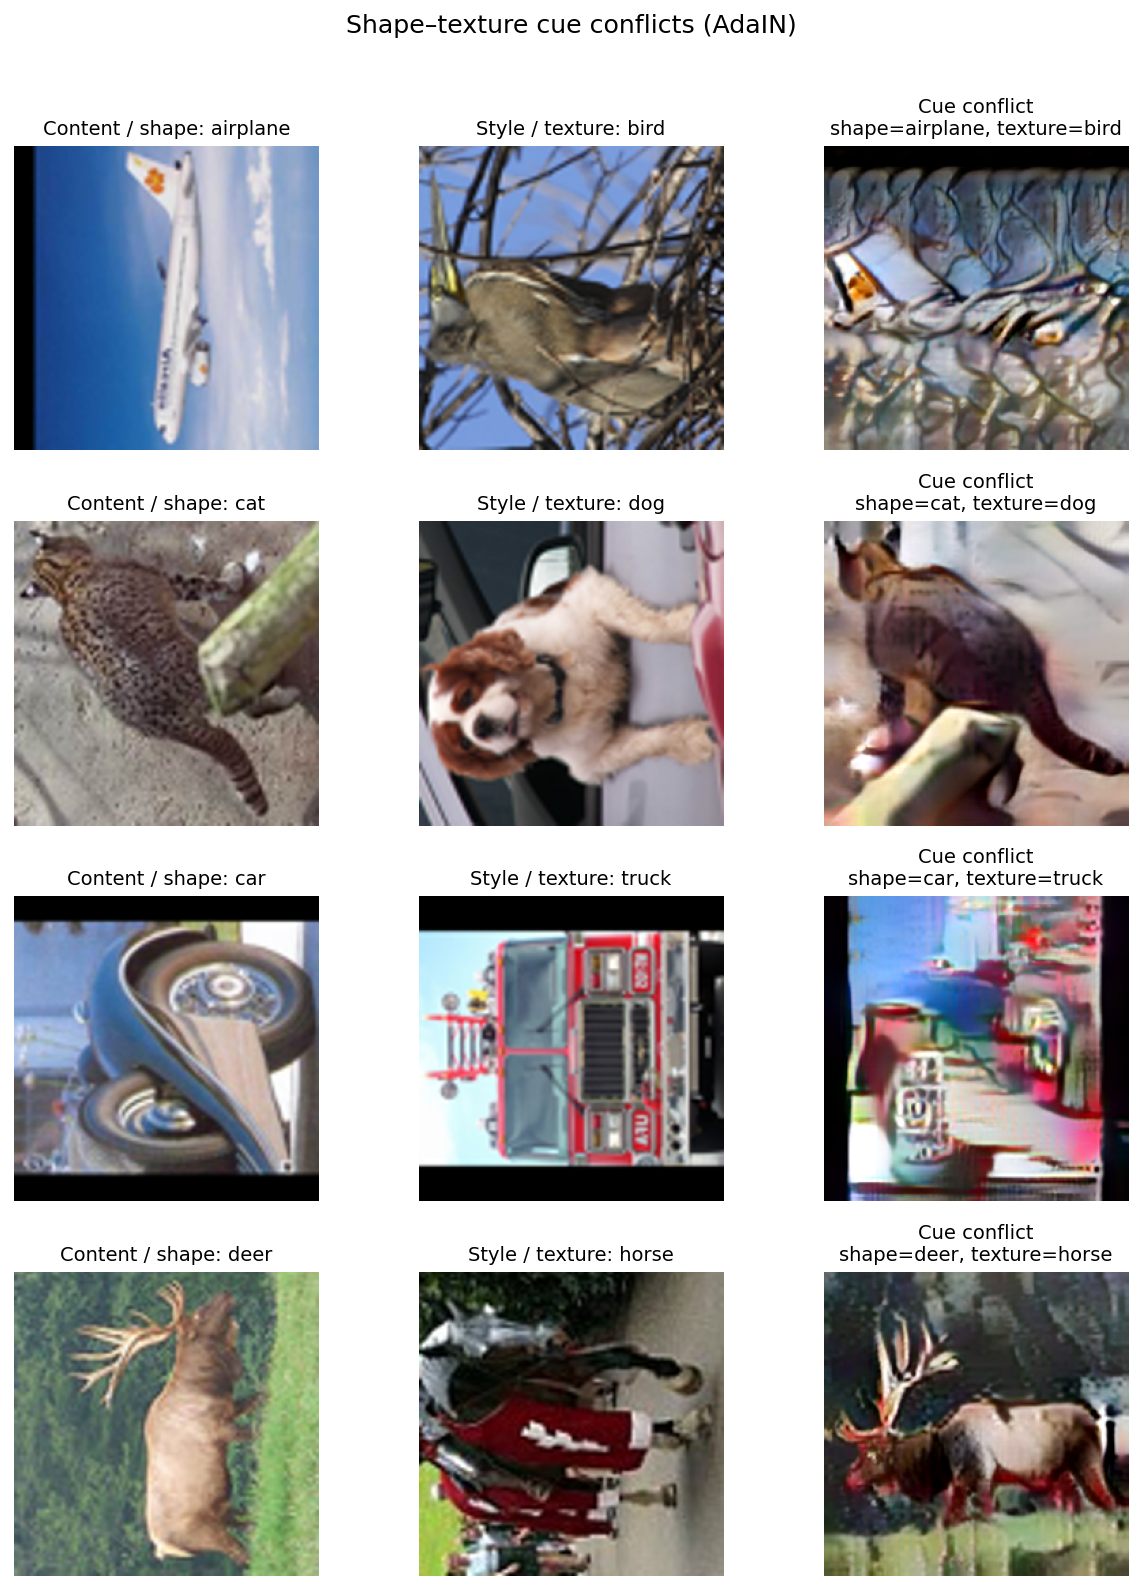
\includegraphics[width=0.92\linewidth]{t1_cue_conflict_examples.png}
  \caption{AdaIN cue conflicts.
  Content supplies shape, style supplies texture.
  The same image can be a shape vote, a texture vote, or neither, which is why coverage belongs next to shape bias.}
  \label{fig:t1_cue_examples}
\end{figure}

\begin{table}[t]
  \centering
  \caption{Cue-conflict counts on $200$ accepted stylizations ($0$ rejected by the visual rule).
  Shape bias ignores the ``other'' column; coverage does not.}
  \label{tab:t1_cue}
  \small
  % Auto-generated by report/scripts/make_report_assets.py. Do not edit by hand.
% Sources: task1/results/tables/task1_summary.json
% accepted conflicts = 200, rejected = 0
\begin{tabular}{lccccc}
\toprule
Model & $N_{\text{shape}}$ & $N_{\text{texture}}$ & $N_{\text{other}}$ & Shape bias (\%) & Coverage (\%) \\
\midrule
ResNet-50 (head) & 91 & 57 & 52 & 61.5 & 74.0 \\
ViT-B/16 (head) & 119 & 36 & 45 & 76.8 & 77.5 \\
CLIP ViT-B/32 (head) & 129 & 17 & 54 & 88.4 & 73.0 \\
CLIP ViT-B/32 (zero-shot) & 117 & 27 & 56 & 81.2 & 72.0 \\
\bottomrule
\end{tabular}

\end{table}

\paragraph{Small translations barely matter. Breaking layout does.}
Write $T_\delta(x)=x+\delta$.
$f$ is translation-invariant if $f(T_\delta(x))=f(x)$ and translation-equivariant if $f(T_\delta(x))=T_\delta(f(x))$.
Pooling gives a CNN some of the first.
A ViT has neither, because of fixed patches and $E_{\mathrm{pos}}$.
The local-versus-global contrast is
\begin{equation}
  y_i=\sum_{j\in\mathcal{L}(i)}w_{i-j}\,x_j
  \quad\text{versus}\quad
  y_i=\sum_{j\in G}A_{ij}\,x_j,
  \label{eq:conv-attn}
\end{equation}
a fixed neighbourhood $\mathcal{L}(i)$ against an input-dependent sum over the whole set $G$.
Figure~\ref{fig:t1_translation} is almost flat through $\delta=32$ for every head (full numbers in Appendix Table~\ref{tab:t1_translation}), so~\eqref{eq:stable} holds for this $T_\delta$ at the prediction level.
There is no CNN-versus-ViT story in those curves.
Patch shuffle is a permutation $T_\pi$ of the $4\times4$ tiles.
Ordinary self-attention is permutation-equivariant, not permutation-invariant, and a ViT with $E_{\mathrm{pos}}$ is not $T_\pi$-invariant.
That is the test of whether $z$ needs the global arrangement in~\eqref{eq:conv-attn}.
Accuracy falls $7.4$ (ViT) and $8.2$ (ResNet) points, and $16.8$ / $15.8$ points for the two CLIP classifiers (Table~\ref{tab:t1_interventions}).
The t-SNE of clean versus shuffled features (Figure~\ref{fig:t1_tsne}) makes the same point in representation space: class clouds smear, and CLIP's cloud smears more.
Mean cosine stability of $z$ under the $4\times4$ shuffle is $0.74$ (CLIP), $0.72$ (ResNet), $0.65$ (ViT).
CLIP's visual features are more committed to ``which patch sits where''.
That is a reasonable inductive bias for a contrastive image--text model, and a liability once the patches are permuted.

\begin{figure}[t]
  \centering
  \begin{minipage}[t]{0.48\linewidth}
    \centering
    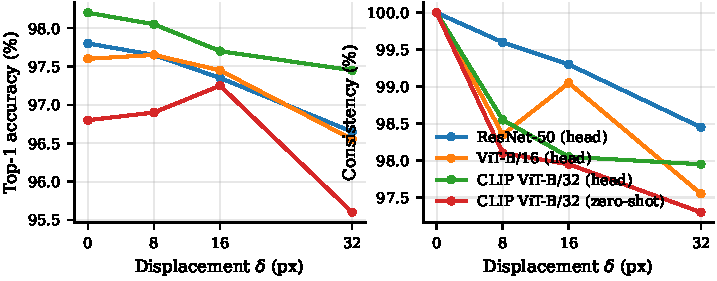
\includegraphics[width=\linewidth]{t1_translation.pdf}
    \caption{Accuracy and consistency under cardinal translations.
    All four heads stay close to clean through $32$ pixels.}
    \label{fig:t1_translation}
  \end{minipage}\hfill
  \begin{minipage}[t]{0.50\linewidth}
    \centering
    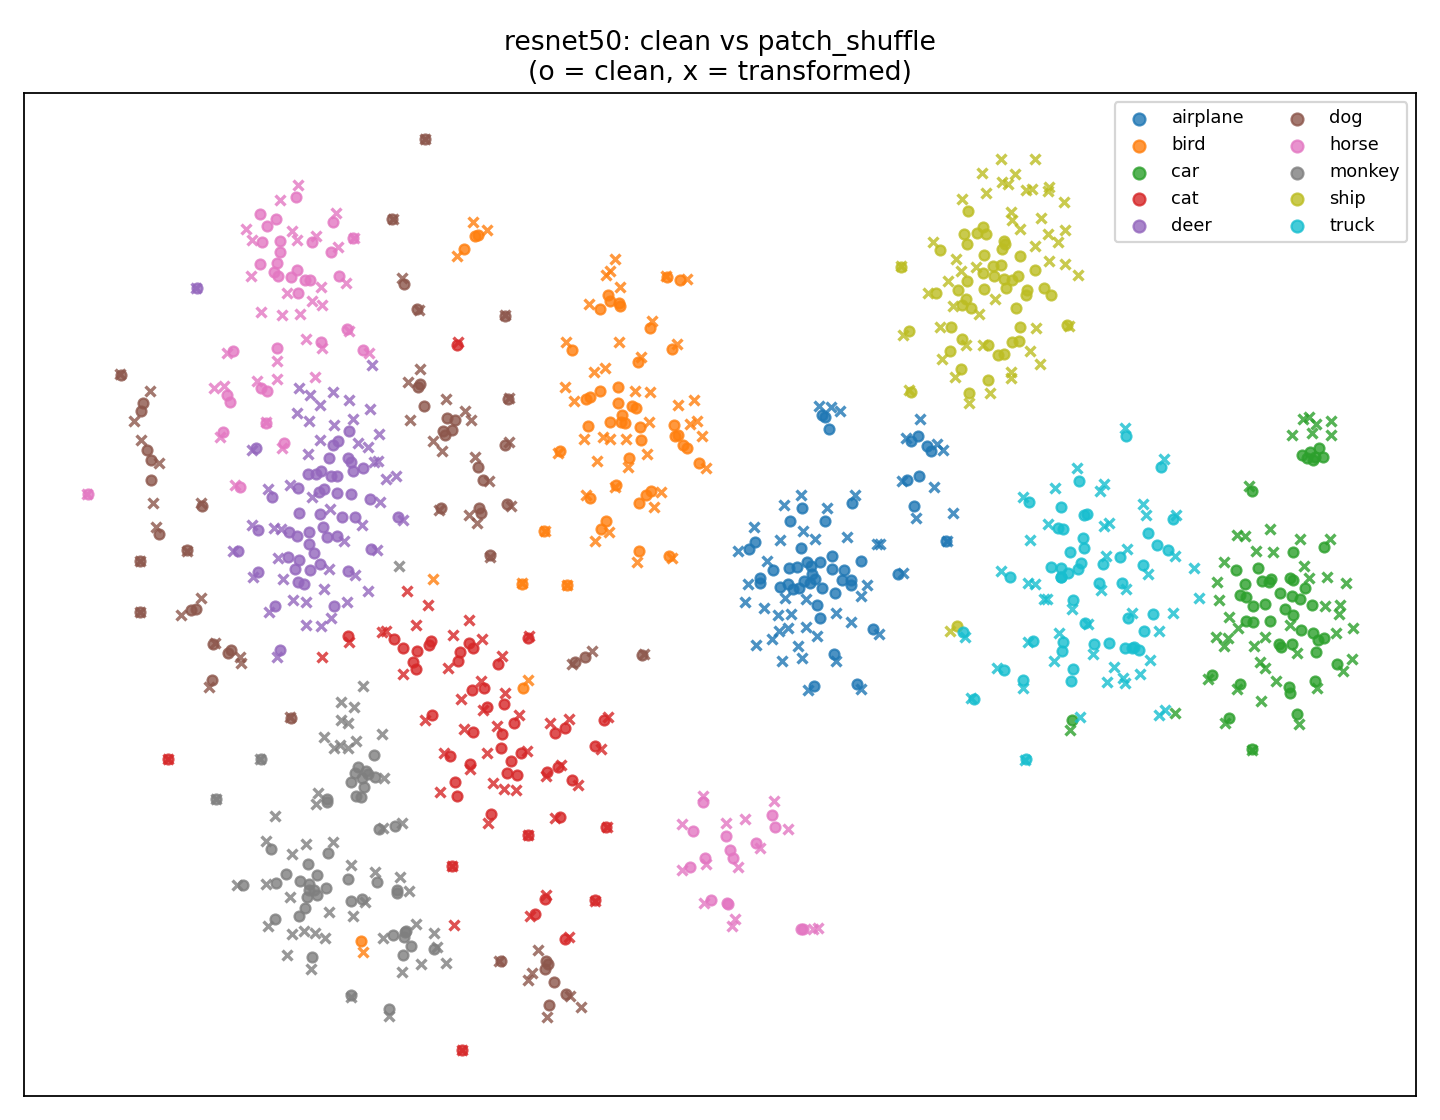
\includegraphics[width=0.32\linewidth]{t1_tsne_resnet50_shuffle.png}\hfill
    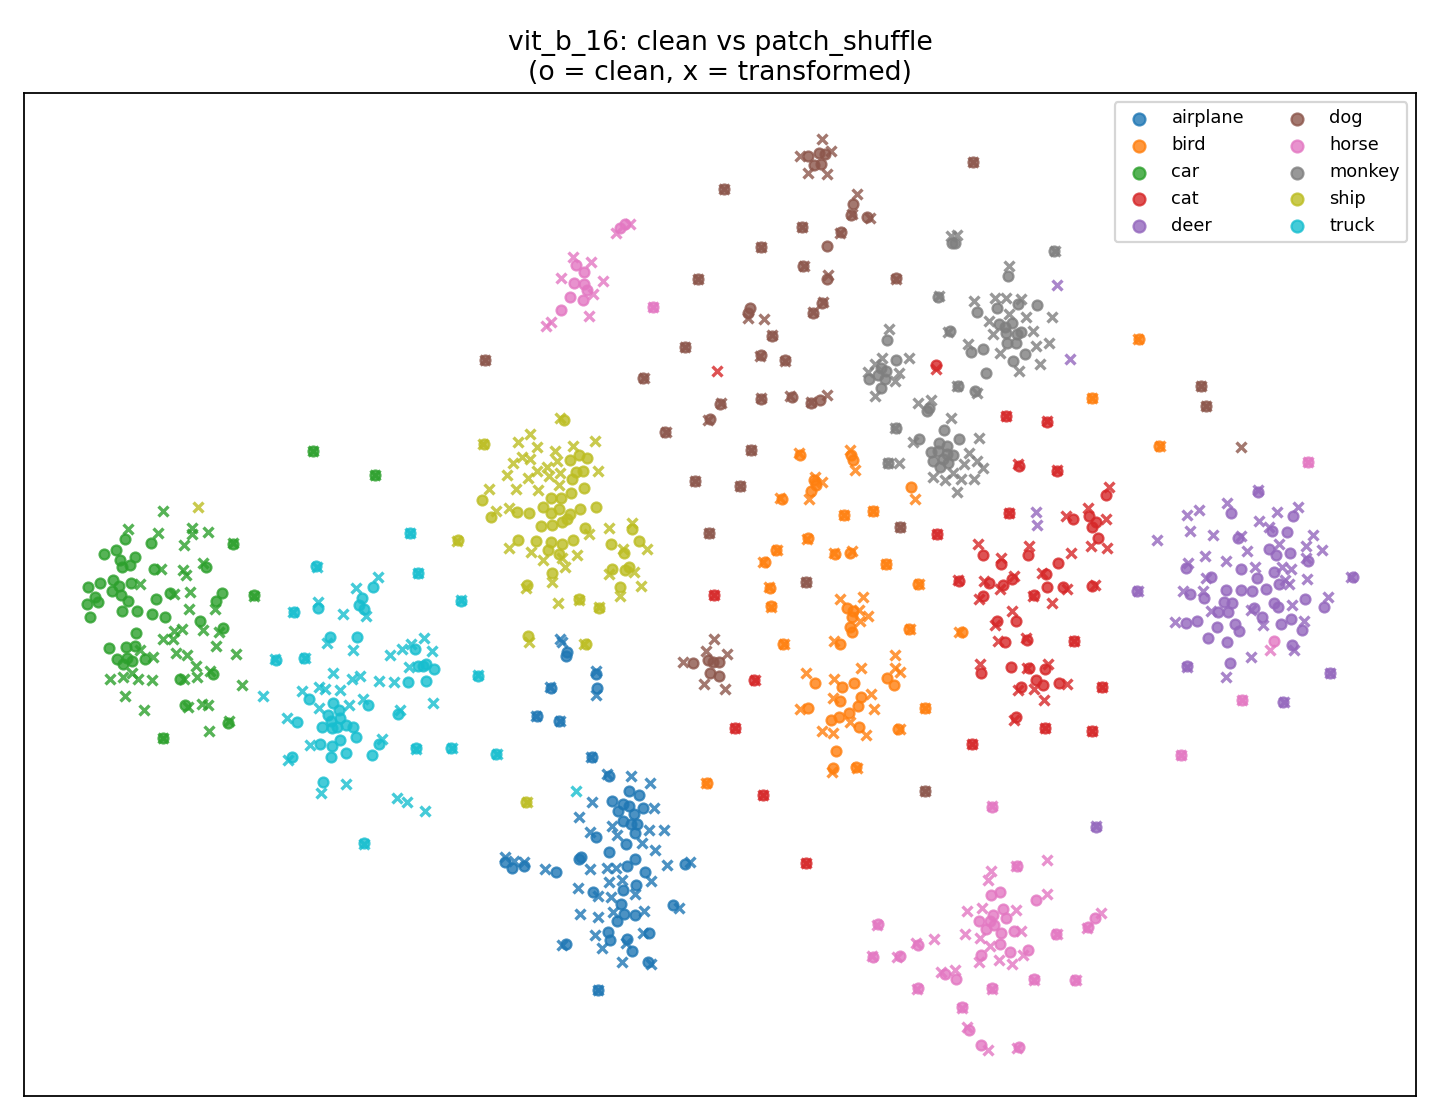
\includegraphics[width=0.32\linewidth]{t1_tsne_vit_shuffle.png}\hfill
    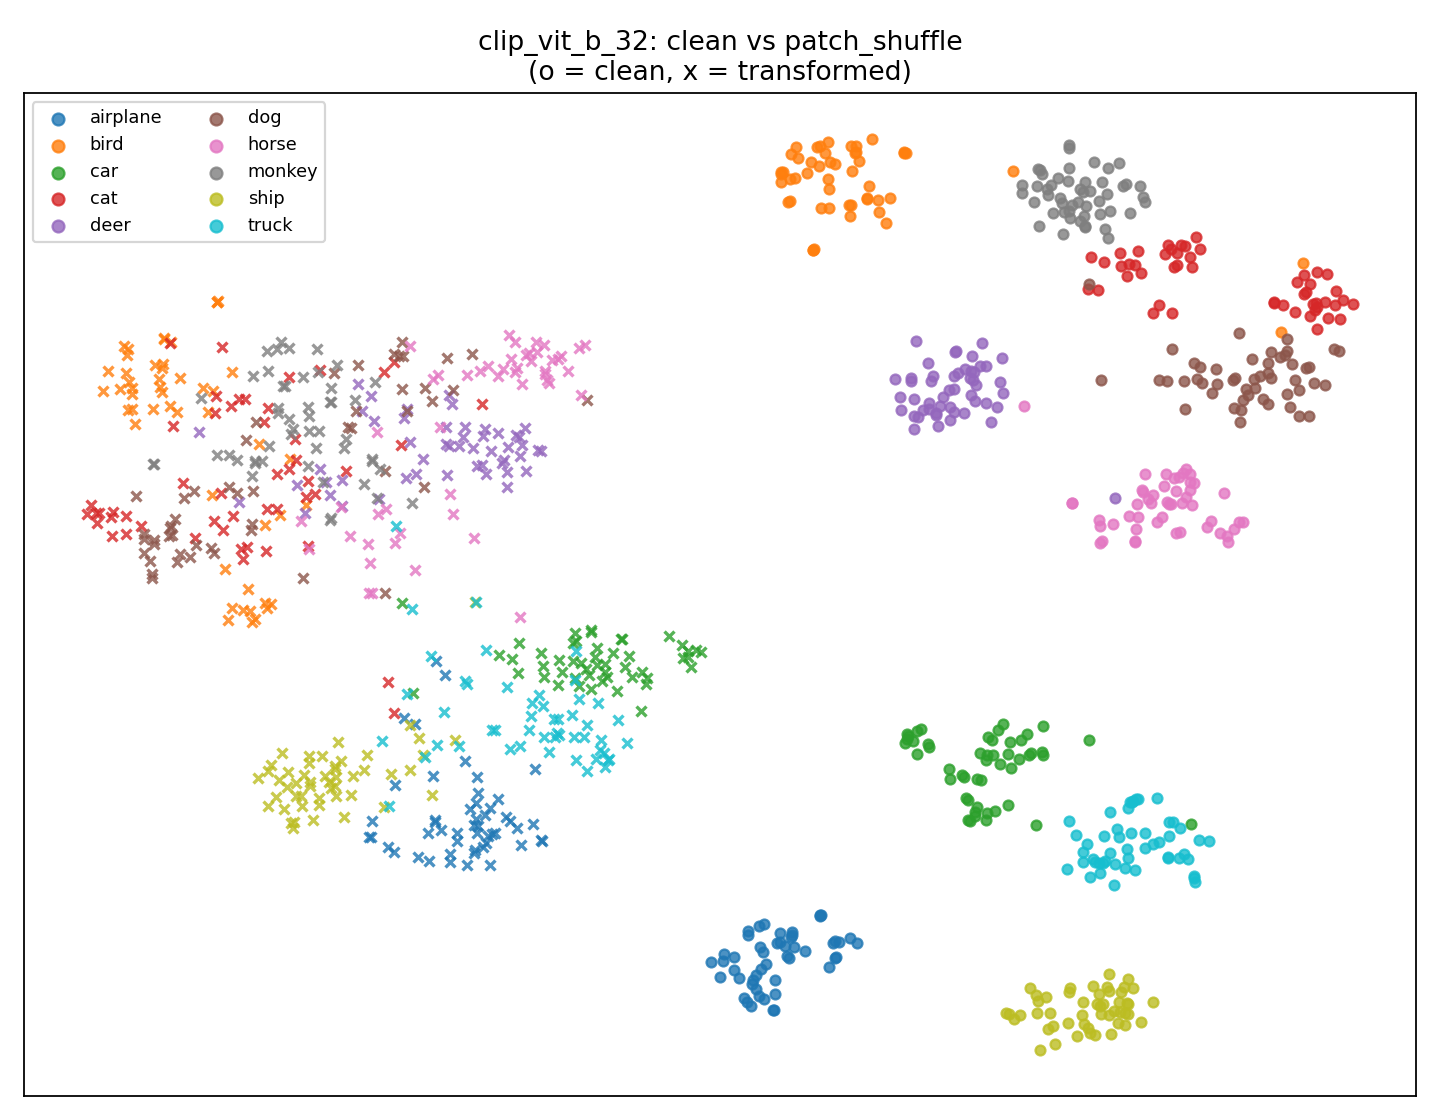
\includegraphics[width=0.32\linewidth]{t1_tsne_clip_shuffle.png}
    \caption{Clean (circles) vs.\ $4\times4$-shuffled (crosses) features.
    CLIP moves the most.
    Grayscale embeddings: Appendix Figure~\ref{fig:t1_tsne_gray}.}
    \label{fig:t1_tsne}
  \end{minipage}
\end{figure}

\paragraph{The head and the embedding do not always vote together.}
Equation~\eqref{eq:stable} is a statement about $z$, not about $\hat y$.
Table~\ref{tab:t1_stability} measures it as mean $\cos\big(z(x),z(T(x))\big)$.
ViT grayscale is the clean mismatch: accuracy drops only $2.0$ points, yet cosine stability is $0.739$.
The linear head can keep the label while $z$ walks.
Cue-conflict stability goes the other way.
ResNet and ViT features of a stylized image sit far from the content image ($0.35$ and $0.31$), while CLIP stays closer ($0.71$), which matches CLIP's higher shape bias.
Zero-shot CLIP and the CLIP linear head share the visual encoder, so their intervention ranking agrees.
They disagree on individual cue-conflict images (the linear head is more shape-loyal; zero-shot more often says ``other'').
A prompt is not the same decision surface as a trained $\psi$.

\begin{table}[t]
  \centering
  \caption{Mean cosine stability of $z$ under each intervention.
  Translation uses a single $16$~px right shift.
  CLIP zero-shot is omitted: it shares the CLIP visual features.}
  \label{tab:t1_stability}
  \small
  % Auto-generated by report/scripts/make_report_assets.py. Do not edit by hand.
% Sources: task1/results/tables/task1_summary.json
% note: Translation stability uses a single representative shift (16px right).
% note: Cue-conflict stability compares stylized features to the content image features.
% note: CLIP zeroshot uses the same visual features as clip_vit_b_32, so it is omitted here.
\begin{tabular}{lcccc}
\toprule
Backbone & Grayscale & Cue conflict & Translation (16 px) & Patch shuffle \\
\midrule
ResNet-50 (head) & 0.788 & 0.351 & 0.944 & 0.715 \\
ViT-B/16 (head) & 0.739 & 0.314 & 0.975 & 0.653 \\
CLIP ViT-B/32 (head) & 0.893 & 0.712 & 0.966 & 0.736 \\
\bottomrule
\end{tabular}

\end{table}

\section{Aligning to an unlabeled target}
\label{sec:uda}

PACS asks for the same seven classes under four styles (Appendix Figure~\ref{fig:t2_pacs}).
Source-only ERM already has the covariate-shift gap in numerical form (Table~\ref{tab:t2_main}): mean source-val accuracy $93.7$, Sketch $66.5$.
Giraffe is the class the source model does not know how to draw ($32.9$); guitar is already fine ($95.9$).
A domain probe on frozen $512$-d features scores $99.6\%$ (chance $50\%$).
$z$ still knows which images are Sketch.

\paragraph{A moderate MMD term uses that unlabeled Sketch.}
DAN is~\eqref{eq:dan} on one layer, the $512$-d feature:
\begin{equation}
  L_{\mathrm{Total}}
  =\mathcal{L}_{CE}(D_S)
  +\lambda_{\mathrm{MMD}}\,\widehat{\mathrm{MMD}}^2(z_S,z_T).
  \label{eq:dan-run}
\end{equation}
At $\lambda_{\mathrm{MMD}}=1$, Sketch rises to $74.9$ ($+8.3$) and source F1 does not fall (Table~\ref{tab:t2_main}).
Domain separability drops from $99.6$ to $95.2$, not to chance.
Figure~\ref{fig:t2_tsne_domain} (center) is that compromise in feature space: source and Sketch occupy the same region.
The class-colored view (Appendix Figure~\ref{fig:t2_tsne_so}, right) still has clusters.
Giraffe collects most of the gain ($+34.9$ points, Table~\ref{tab:t23_perclass}).
House and person go up as well; dog slips a little.
This is the case where shrinking the middle term of~\eqref{eq:da-bound} helps $L_T$ while $L_S$ in~\eqref{eq:ce} stays small.
The probe is still $95.2\%$, so $\min(a,b)$ was not driven to zero; it just did not get worse enough to cancel the gain.

\begin{table}[t]
  \centering
  \caption{PACS unsupervised DA.
  Source columns are validation Acc / macro-F1.
  Domain separability is a held-out logistic probe (chance $50\%$).
  $\Delta$Acc is Sketch accuracy minus source-only.}
  \label{tab:t2_main}
  \small\setlength{\tabcolsep}{3.5pt}
  % Auto-generated by report/scripts/make_report_assets.py. Do not edit by hand.
% Sources: task2/results/tables/task2_main_comparison.json
\begin{tabular}{lccccccccc}
\toprule
 & \multicolumn{3}{c}{Source val. (Acc / F1)} & \multicolumn{2}{c}{Mean source} & \multicolumn{3}{c}{Sketch (target)} & \\
\cmidrule(lr){2-4}\cmidrule(lr){5-6}\cmidrule(lr){7-9}
Method & P & A & C & Acc & F1 & Acc & F1 & $\Delta$Acc & Dom. sep. \\
\midrule
Source-only (ERM) & 97.6 / 97.1 & 89.5 / 88.7 & 94.0 / 94.1 & 93.7 & 93.3 & 66.5 & 68.3 & $+0.0$ & 99.6 \\
DAN ($\lambda_{\text{MMD}}=1$) & 97.6 / 97.1 & 91.2 / 91.0 & 93.8 / 94.5 & 94.2 & 94.2 & 74.9 & 72.4 & $+8.3$ & 95.2 \\
DANN & 96.7 / 96.2 & 91.7 / 91.9 & 94.7 / 95.1 & 94.4 & 94.4 & 27.4 & 34.2 & $-39.1$ & 99.5 \\
CDAN & 96.7 / 96.1 & 93.7 / 93.2 & 94.2 / 94.9 & 94.9 & 94.7 & 53.1 & 55.4 & $-13.4$ & 99.0 \\
\bottomrule
\end{tabular}

\end{table}

\paragraph{A discriminator on $z$ can look aligned on the source loss and still destroy Sketch.}
DANN trains~\eqref{eq:dann} through~\eqref{eq:grl}.
Source accuracy stays $94.4$ ($L_S$ is fine) and Sketch is $27.4$ ($-39.1$).
Domain separability stays $99.5$, so the middle term of~\eqref{eq:da-bound} did not even fall.
Figure~\ref{fig:t2_tsne_domain} (right) is why: Sketch is a tight island, sources sit in rings around it.
The reversed gradient moved $z$ in a way that kept $D_{\theta_d}$ busy and wrecked $s_j$ on Sketch.
The dominant confusions are dog, horse, elephant, giraffe, and even guitar into \emph{person} (Table~\ref{tab:t23_confusions}).
A min-max game can over-align, and a single discriminator on marginals can wrongly align conditionals: $\min(a,b)$ grew.
CDAN keeps~\eqref{eq:grl} but replaces $z$ by $g(x)=\mathrm{vec}(f\otimes p)$.
It is better than DANN ($53.1$) and worse than doing nothing.
Soft $p$ on a moving Sketch feature is a noisy class name.
Animals collapse into horse instead of person (Table~\ref{tab:t23_confusions}).
Conditioning on the head does not create class-conditional alignment if the head is already confused.

The class-colored DANN plot (Appendix Figure~\ref{fig:t2_tsne_dann}) is a smear.
CDAN's matching embeddings are Appendix Figure~\ref{fig:t2_tsne_dann} (right).

Training curves (Figure~\ref{fig:t2_curves}) add a time axis.
Source-only CE falls and source F1 rises, then early-stops.
DAN's MMD term drops while source F1 stays high.
DANN and CDAN keep a large domain loss and a high source F1: the head is still solving Photo / Art / Cartoon while $z$ is being pulled by a reversed gradient that Sketch never supervises.

\begin{figure}[t]
  \centering
  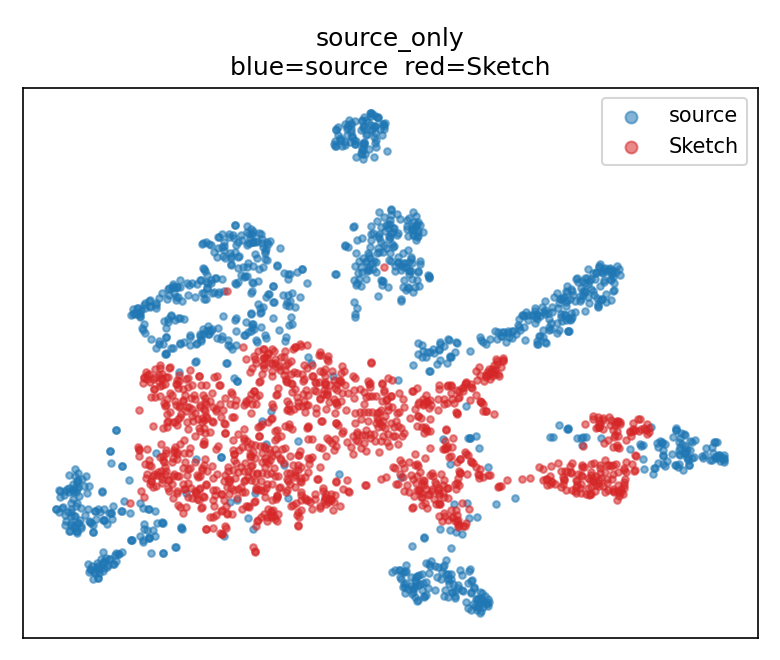
\includegraphics[width=0.32\linewidth]{t2_tsne_domain_source_only.png}\hfill
  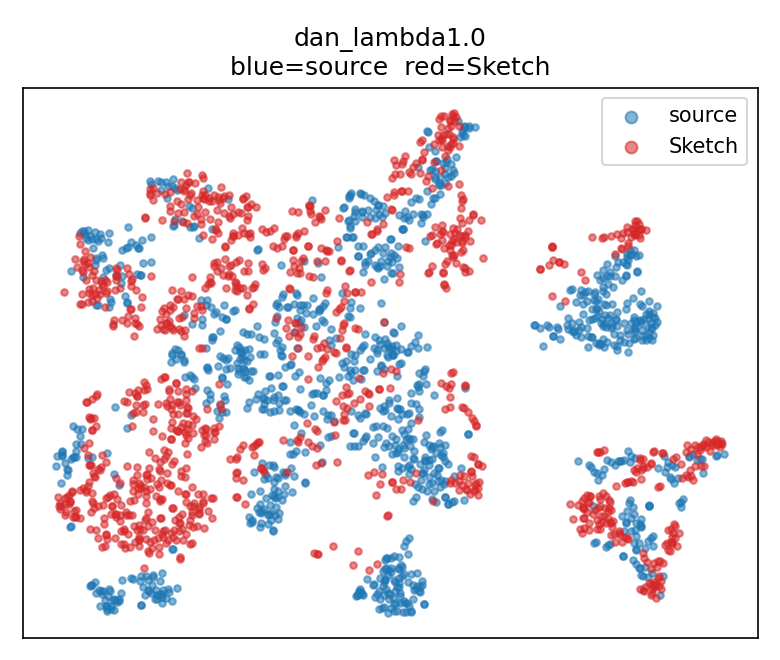
\includegraphics[width=0.32\linewidth]{t2_tsne_domain_dan_lam1.png}\hfill
  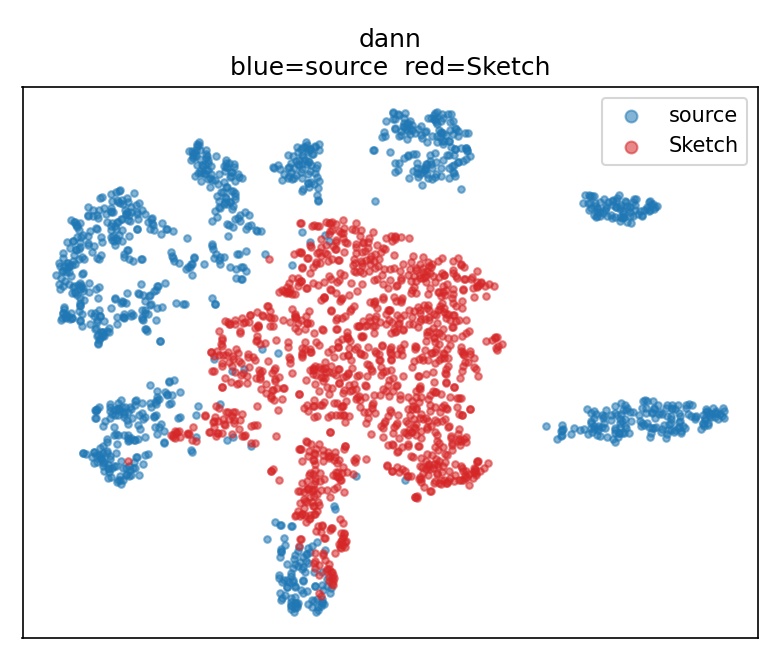
\includegraphics[width=0.32\linewidth]{t2_tsne_domain_dann.png}
  \caption{Learned $512$-d features, domain-colored (blue source, red Sketch), same $450{+}450$ subset.
  Left: ERM, Sketch is its own blob.
  Middle: DAN $\lambda{=}1$, the clouds mix.
  Right: DANN, Sketch is isolated again.
  Class-colored versions are Appendix Figure~\ref{fig:t2_tsne_so}.}
  \label{fig:t2_tsne_domain}
\end{figure}

\begin{figure}[t]
  \centering
  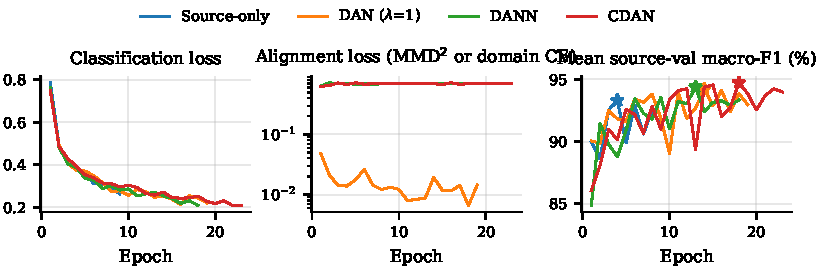
\includegraphics[width=0.88\linewidth]{t2_curves.pdf}
  \caption{Task~2 training.
  Alignment loss is MMD$^2$ for DAN and domain CE for DANN / CDAN.
  High source F1 is cheap; Sketch is not in this plot.}
  \label{fig:t2_curves}
\end{figure}

\paragraph{$\lambda_{\mathrm{MMD}}$ is not ``more invariance is better''.}
Table~\ref{tab:t2_lambda} is the controlled study, chosen before looking at Sketch.
$\lambda=0.1$ is source-only in disguise (Sketch $66.2$, separability $99.5$).
$\lambda=1$ is the useful point.
$\lambda=10$ lowers separability further ($93.0$) and also drops source F1 to $87.5$; Sketch falls back to $67.6$.
Centroid $\ell_2$ between mean source and mean Sketch features is smallest at $\lambda=1$ ($13.3$), not at $\lambda=10$ ($40.4$).
Strong MMD can move means in a way that is not useful.
If Sketch labels had been hidden, $\lambda=1$ is still the setting I would keep: best source F1 among the three, and the first visible drop in the domain probe.
Separability alone would have picked $\lambda=10$ and thrown away the classifier.
Appendix Figure~\ref{fig:t2_lambda_curves} shows the same $\lambda$ runs over epochs; Appendix Figure~\ref{fig:t2_tsne_lam10} is the $\lambda=10$ embedding.

\begin{table}[t]
  \centering
  \caption{DAN alignment pressure.
  Centroid $\ell_2$ is the distance between the mean source-val feature and the mean Sketch feature on the t-SNE diagnostic subset.}
  \label{tab:t2_lambda}
  \small
  % Auto-generated by report/scripts/make_report_assets.py. Do not edit by hand.
% Sources: task2/results/tables/task2_lambda_study.json, task2/results/figures/feature_tsne/centroid_distances.json
% centroid L2 = distance between mean source-val and mean Sketch feature (450 each), from the t-SNE diagnostic
\begin{tabular}{cccccccc}
\toprule
$\lambda_{\text{MMD}}$ & Src Acc & Src F1 & Dom. sep. & Centroid $\ell_2$ & Sketch Acc & Sketch F1 & $\Delta$Acc \\
\midrule
0.1 & 93.9 & 93.9 & 99.5 & 24.1 & 66.2 & 66.5 & $-0.4$ \\
1 & 94.2 & 94.2 & 95.2 & 13.3 & 74.9 & 72.4 & $+8.3$ \\
10 & 87.8 & 87.5 & 93.0 & 40.4 & 67.6 & 67.7 & $+1.1$ \\
\bottomrule
\end{tabular}

\end{table}

\section{Generalizing with no target access}
\label{sec:dg}

Equation~\eqref{eq:dg-bound} leaves three moves: lower every source risk, shrink the source--source radius $\rho$, and hope $P_T$ still sits in $\Lambda$.
Sketch is unseen in training, selection, and the source diagnostics.
The ERM row in Table~\ref{tab:t3_main} is the same $66.5$ Sketch number as Table~\ref{tab:t2_main}.
That is the hinge for the comparison.

\begin{table}[t]
  \centering
  \caption{Domain generalization on the same PACS split.
  Source separability is a $3$-way probe (chance $33\%$), not the Task~2 source-versus-Sketch probe.
  $\Delta_{\mathrm{sharp}}=L(\theta+\bar\epsilon)-L(\theta)$ at $\rho=0.05$.}
  \label{tab:t3_main}
  \small\setlength{\tabcolsep}{2.5pt}
  \resizebox{\linewidth}{!}{% Auto-generated by report/scripts/make_report_assets.py. Do not edit by hand.
% Sources: task3/results/tables/task3_main_comparison.json
\begin{tabular}{lccccccccc}
\toprule
 & \multicolumn{5}{c}{Source validation (Acc / F1)} & & & & \\
\cmidrule(lr){2-6}
Method & P & A & C & Mean & Worst & Sketch (Acc / F1) & $\Delta$Acc & Src sep. & $\Delta_{\text{sharp}}$ \\
\midrule
ERM (Task 2 source-only) & 97.6 / 97.1 & 89.5 / 88.7 & 94.0 / 94.1 & 93.7 / 93.3 & 89.5 / 88.7 & 66.5 / 68.3 & $+0.0$ & 89.7 & 0.317 \\
DAN-DG ($\lambda_{\text{DG}}=1$) & 96.1 / 95.3 & 88.3 / 88.4 & 93.4 / 94.2 & 92.6 / 92.7 & 88.3 / 88.4 & 63.1 / 63.5 & $-3.4$ & 78.1 & 0.258 \\
SAM ($\rho=0.05$) & 97.0 / 96.5 & 93.2 / 93.0 & 94.9 / 95.2 & 95.0 / 94.9 & 93.2 / 93.0 & 44.6 / 48.7 & $-22.0$ & 88.0 & 0.142 \\
\bottomrule
\end{tabular}
}
\end{table}

\paragraph{Making Photo, Art, and Cartoon look alike is not the same as making them look like Sketch.}
DAN-DG attacks the $\rho$ term in~\eqref{eq:dg-bound}, not the $\mathrm{Divergence}(P_S,P_T)$ term in~\eqref{eq:da-bound}:
\begin{equation}
  L_{\mathrm{Total}}
  =\mathcal{L}_{CE}
  +\lambda_{\mathrm{DG}}\cdot
  \tfrac13\big(\widehat{\mathrm{MMD}}^2_{PA}+\widehat{\mathrm{MMD}}^2_{PC}+\widehat{\mathrm{MMD}}^2_{AC}\big).
  \label{eq:dan-dg}
\end{equation}
The three sources are Photo, Art, Cartoon.
$\lambda_{\mathrm{DG}}=1$.
Three-way source separability falls from $89.7$ to $78.1$.
Mean source F1 slips from $93.3$ to $92.7$.
Sketch goes the wrong way: $63.1$ ($-3.4$).
Elephant jumps ($+19.5$); dog collapses ($-26.0$); house drops $16$ points (Table~\ref{tab:t23_perclass}).
The invariance is real and it is not the invariance Sketch needed.
At $\lambda_{\mathrm{DG}}=10$ the method says this out loud (Table~\ref{tab:t3_lambda}): source F1 $12.2$, Sketch $24.5$, and the confusion matrix is almost ``predict dog''.
That is~\eqref{eq:dan-dg} eating the true-class logits in~\eqref{eq:ce}, plus $\gamma(P_T,\Lambda)$ in~\eqref{eq:dg-bound} left untouched because Sketch was never in the MMD.
Appendix Figure~\ref{fig:t3_lambda_curves} is the training view: the MMD term dies, CE does not.

\begin{table}[t]
  \centering
  \caption{DAN-DG alignment pressure, no Sketch in the batch.
  $\lambda_{\mathrm{DG}}=10$ is a collapsed source classifier, not a stronger invariant one.}
  \label{tab:t3_lambda}
  \small
  % Auto-generated by report/scripts/make_report_assets.py. Do not edit by hand.
% Sources: task3/results/tables/task3_lambda_study.json
\begin{tabular}{ccccccc}
\toprule
$\lambda_{\text{DG}}$ & Mean src F1 & Worst src F1 & Src sep. & $\Delta_{\text{sharp}}$ & Sketch Acc & Sketch F1 \\
\midrule
0.1 & 94.2 & 91.8 & 84.4 & 0.370 & 62.2 & 65.8 \\
1 & 92.7 & 88.4 & 78.1 & 0.258 & 63.1 & 63.5 \\
10 & 12.2 & 10.5 & 73.1 & 3.684 & 24.5 & 10.0 \\
\bottomrule
\end{tabular}

\end{table}

\paragraph{A flatter source bowl is not a Sketch bowl.}
SAM is~\eqref{eq:sam} with $\rho=0.05$.
It does what it is paid to do.
$\Delta_{\mathrm{sharp}}=L(\theta+\bar\epsilon)-L(\theta)$ falls from $0.317$ (ERM) to $0.142$.
Mean source F1 is the best of the three ($94.9$), and the worst source domain (Art) improves.
Sketch is $44.6$ ($-22.0$).
Horse and guitar, two classes ERM already handled, fall by about $55$ points each (Table~\ref{tab:t23_perclass}).
SAM for DG is hard because domains need not share a flat region.
Here the ranking is inverted: the flattest source solution is the worst unseen-domain solution.
Mean and worst source-val F1 would have selected SAM and rejected the ERM checkpoint that is $22$ points better on Sketch.
Figure~\ref{fig:t3_curves} is the training picture.
SAM's perturbed CE keeps falling; DAN-DG's MMD falls while source F1 stays ordinary.

\begin{figure}[t]
  \centering
  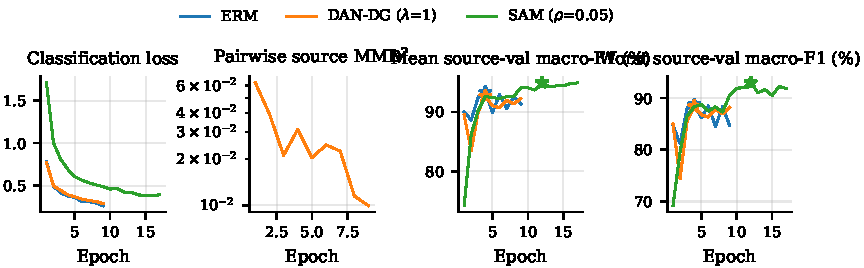
\includegraphics[width=0.88\linewidth]{t3_curves.pdf}
  \caption{Task~3 training on sources only.
  DAN-DG logs CE and pairwise MMD.
  SAM logs CE at $\theta+\bar\epsilon$.
  Source F1 is the only selection signal.}
  \label{fig:t3_curves}
\end{figure}

\paragraph{Per-class, the two alignment graphs do not edit the same animals.}
Table~\ref{tab:t23_perclass} and Appendix Figure~\ref{fig:perclass_delta} put Task~2 and Task~3 on one grid.
Target-aware DAN repairs giraffe.
Target-free DAN-DG repairs elephant and damages dog.
SAM repairs almost nothing that matters and deletes horse and guitar.
Table~\ref{tab:t23_confusions} is the failure mode in words: ERM mixes giraffes and horses with dogs; DANN dumps animals into person; CDAN dumps them into horse; SAM dumps horses and giraffes into dog.
The shared ERM is the only fair hinge for ``what unlabeled Sketch contributed''.
Against that hinge, DAN is $+8.3$ and DAN-DG is $-3.4$.
That is not a causal claim that ``target access'' is the only difference.
The alignment graph, the bandwidth sample (24 Sketch images versus three pairs of 8), and the selected epoch (14 versus 4) all change.
It is still the comparison the protocol was built for, and it goes in one direction.

\begin{table}[t]
  \centering
  \caption{Sketch per-class accuracy and change versus ERM.
  $n$ is the number of Sketch images.
  DAN sees unlabeled Sketch; DAN-DG and SAM do not.}
  \label{tab:t23_perclass}
  \small\setlength{\tabcolsep}{3.5pt}
  % Auto-generated by report/scripts/make_report_assets.py. Do not edit by hand.
% Sources: task2/results/tables/eval_source_only_best.json, task2/results/tables/eval_dan_lambda1.0_best.json, task2/results/tables/eval_dann_best.json, task2/results/tables/eval_cdan_best.json, task3/results/tables/eval_dan_dg_lambda1.0.json, task3/results/tables/eval_sam_rho0.05.json
% cells: Sketch per-class accuracy (change vs ERM), in percent; (n) = Sketch images per class
\begin{tabular}{lcccccc}
\toprule
 & & \multicolumn{3}{c}{Task 2 (sees unlabeled Sketch)} & \multicolumn{2}{c}{Task 3 (Sketch unseen)} \\
\cmidrule(lr){3-5}\cmidrule(lr){6-7}
Class ($n$) & ERM & DAN & DANN & CDAN & DAN-DG & SAM \\
\midrule
dog (772) & 59.3 & 56.9 ($-2.5$) & 6.6 ($-52.7$) & 14.2 ($-45.1$) & 33.3 ($-26.0$) & 66.6 ($+7.3$) \\
elephant (740) & 76.6 & 80.3 ($+3.6$) & 23.9 ($-52.7$) & 26.1 ($-50.5$) & 96.1 ($+19.5$) & 69.1 ($-7.6$) \\
giraffe (753) & 32.9 & 67.9 ($+34.9$) & 20.5 ($-12.5$) & 22.3 ($-10.6$) & 31.9 ($-1.1$) & 23.0 ($-10.0$) \\
guitar (608) & 95.9 & 92.6 ($-3.3$) & 55.9 ($-40.0$) & 97.4 ($+1.5$) & 87.8 ($-8.1$) & 41.0 ($-54.9$) \\
horse (816) & 68.6 & 73.4 ($+4.8$) & 15.9 ($-52.7$) & 97.2 ($+28.6$) & 69.2 ($+0.6$) & 12.9 ($-55.8$) \\
house (80) & 81.2 & 100.0 ($+18.8$) & 91.2 ($+10.0$) & 98.8 ($+17.5$) & 65.0 ($-16.2$) & 80.0 ($-1.2$) \\
person (160) & 83.1 & 96.9 ($+13.7$) & 95.6 ($+12.5$) & 95.0 ($+11.9$) & 76.2 ($-6.9$) & 84.4 ($+1.2$) \\
\bottomrule
\end{tabular}

\end{table}

\begin{table}[t]
  \centering
  \caption{Top Sketch confusions (true $\to$ predicted, count).}
  \label{tab:t23_confusions}
  \small
  % Auto-generated by report/scripts/make_report_assets.py. Do not edit by hand.
% Sources: task2/results/tables/eval_source_only_best.json, task2/results/tables/eval_dan_lambda1.0_best.json, task2/results/tables/eval_dann_best.json, task2/results/tables/eval_cdan_best.json, task3/results/tables/eval_dan_dg_lambda1.0.json, task3/results/tables/eval_sam_rho0.05.json
\begin{tabular}{llll}
\toprule
Model & 1st & 2nd & 3rd \\
\midrule
ERM & giraffe$\to$dog (189) & horse$\to$dog (159) & giraffe$\to$horse (150) \\
DAN & dog$\to$person (156) & dog$\to$elephant (88) & giraffe$\to$dog (87) \\
DANN & dog$\to$person (609) & horse$\to$person (606) & elephant$\to$person (557) \\
CDAN & dog$\to$horse (481) & elephant$\to$horse (454) & giraffe$\to$horse (431) \\
DAN-DG & dog$\to$elephant (297) & giraffe$\to$horse (190) & dog$\to$horse (173) \\
SAM & horse$\to$dog (573) & giraffe$\to$dog (351) & guitar$\to$person (278) \\
\bottomrule
\end{tabular}

\end{table}

\section{When the label is new}
\label{sec:osr}

UDA and DG keep $\mathcal{Y}_K$ fixed and move $P(X)$.
OSR keeps $P_K$ and asks for a second output: reject if $x$ looks like $\mathcal{Y}_U$.
Equation~\eqref{eq:ce} never sees an unknown, and far from the training points the decision regions are unbounded cones.
That is how $R_{\mathcal{O}}$ in~\eqref{eq:open-risk} grows: the accepted set walks into $\mathcal{O}$.
False confidence is the symptom, not a separate disease.

\paragraph{Four scores are four different proxies for~\eqref{eq:lrt}.}
On the frozen Vanilla model (Table~\ref{tab:t4_scores})
\begin{align}
  u_{\mathrm{MSP}}(x)&=1-\max_k P_k,
  \label{eq:msp}\\
  u_{\mathrm{MLS}}(x)&=-\max_k z_k,
  \label{eq:mls}\\
  u_{\mathrm{energy}}(x)&=-\log\sum_k e^{z_k},
  \label{eq:energy}\\
  u_{\mathrm{MAH}}(x)&=\min_{c\in\mathcal{Y}_K}(h-\mu_c)^\top\Sigma^{-1}(h-\mu_c).
  \label{eq:mah}
\end{align}
$P_k$ is relative dominance among known classes.
$\max_k z_k$ is the absolute size of the winning logit.
Energy is the log-partition of all logits, so it agrees with MLS when one $z_k$ dominates the sum.
Mahalanobis is distance of $h$ to the nearest known-class cloud, with one shared $\Sigma$.
Far AUROC sits in the high $80$s to low $90$s; near AUROC sits near $80$ for every score.
Rejecting a bowl is easier than rejecting a wolf.
MLS and Energy are almost the same ranking, which they should be when one logit dominates the sum.
Mahalanobis is the best far detector ($92.1$ AUROC) and not special on near ($80.3$): an unknown fox can land next to dog.
MSP's histogram (Figure~\ref{fig:t4_scores}, left) is a spike at $0$.
Most knowns, and too many unknowns, look like $p\approx[1,0,\ldots]$.
High relative confidence is not high evidence of being known.
The val-calibrated point $\tau$ (dashed) is the only operating point that known validation may choose: about $95\%$ of known val examples are kept, and most near unknowns are still accepted (reject $27$--$30\%$).
AUROC and FPR@$95$TPR answer different questions, and both belong in the table.

\begin{table}[t]
  \centering
  \caption{Post-hoc scores on frozen Vanilla.
  $\tau$ is the $95$th percentile of $u$ on CIFAR-10 validation.
  Known acc.\ is CIFAR-10 test acceptance at that $\tau$.}
  \label{tab:t4_scores}
  \small\setlength{\tabcolsep}{4pt}
  % Auto-generated by report/scripts/make_report_assets.py. Do not edit by hand.
% Sources: task4/results/tables/task4_score_comparison.json
\begin{tabular}{lcccccccc}
\toprule
 & \multicolumn{3}{c}{AUROC (\%)} & \multicolumn{3}{c}{At $\tau$ = val. 95th pct. (\%)} & \multicolumn{2}{c}{FPR@95TPR (\%)} \\
\cmidrule(lr){2-4}\cmidrule(lr){5-7}\cmidrule(lr){8-9}
Score $u(x)$ & Near & Far & All & Known acc. & Near rej. & Far rej. & Near & Far \\
\midrule
MSP & 81.5 & 89.5 & 85.5 & 94.7 & 27.3 & 43.0 & 72.8 & 57.0 \\
MLS & 79.8 & 88.7 & 84.3 & 95.4 & 29.4 & 49.4 & 70.6 & 50.6 \\
Energy & 79.9 & 88.8 & 84.3 & 95.4 & 30.5 & 50.6 & 69.5 & 49.4 \\
Mahalanobis & 80.3 & 92.1 & 86.2 & 94.9 & 27.5 & 52.0 & 72.5 & 48.0 \\
\bottomrule
\end{tabular}

\end{table}

\begin{figure}[t]
  \centering
  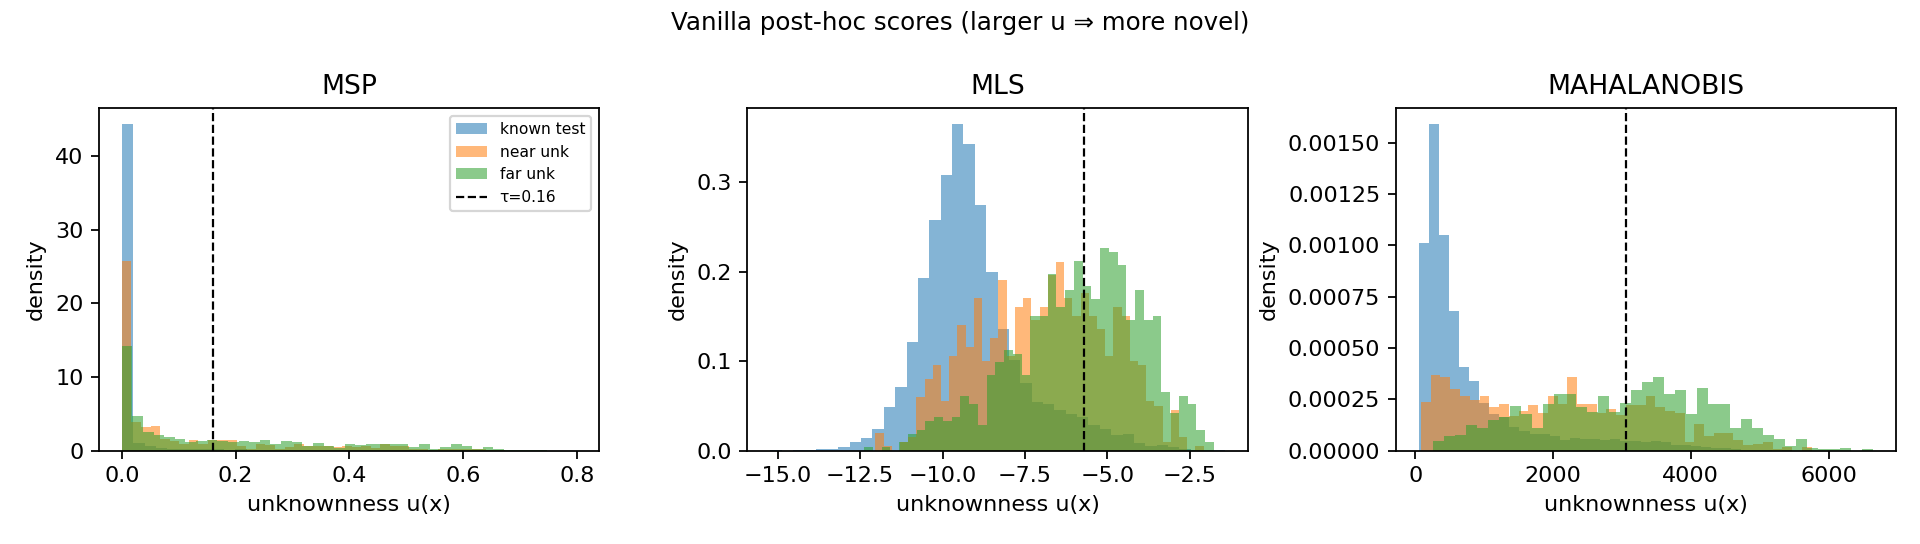
\includegraphics[width=0.92\linewidth]{t4_score_distributions.png}
  \caption{Vanilla unknownness on known test, near, and far CIFAR-100.
  Larger $u$ means more novel.
  MSP piles everyone at zero.
  MLS separates far better than near.
  Mahalanobis stretches far unknowns away from the known peak.}
  \label{fig:t4_scores}
\end{figure}

\paragraph{A slightly better closed-set model is a slightly safer rejector here. A placeholder head is not.}
Table~\ref{tab:t4_models} holds the training axis fixed (MLS) except for the extra PROSER row.
GCSC changes only the augmentation.
CSA goes $94.7\to 95.1$.
Near AUROC $79.8\to 81.5$, far $88.7\to 90.5$, far reject at $\tau$ $49.4\to 60.0$.
In this run the claim that a good closed-set classifier plus MLS is enough is directionally true, and it is more true for far than for near.
The correlation is still empirical: CSA rewards any direction that raises known accuracy, including a texture cue that later fails on a leopard.
PROSER manufactures a proxy unknown~\citep{zhou2021learning}.
Hidden states of two known classes are mixed,
\begin{equation}
  h_u=\lambda h_i+(1-\lambda)h_j,
  \qquad\lambda\sim\mathrm{Beta}(2,2),
  \label{eq:mixup}
\end{equation}
and the extra logit $z_u$ is trained with
\begin{equation}
  \mathcal{L}_{\mathrm{cls}}
  =\ell_{CE}([z,z_u],y_j)
  +\beta\,\ell_{CE}([z\setminus y_j,\,z_u],\,y_{K+1}).
  \label{eq:proser}
\end{equation}
The first term keeps the true class on top.
The second asks the dummy class to win once $y_j$ is masked.
CSA drops to $94.4$.
MLS-AUROC is close to Vanilla and worse than GCSC at the operating point.
The placeholder score, the thing PROSER is supposed to add, is the weakest row in the table (far AUROC $82.8$, far reject $35\%$).
Points on the segment between cat and truck are not sunflowers.
Table~\ref{tab:t4_failures} is the human check at Vanilla MLS ($\tau=-5.72$).
bus$\to$truck and wolf$\to$dog are the near-unknown story.
sunflower$\to$bird and bowl$\to$truck are the generic-feature story: $h$ that separates known classes from each other is still true of things outside $\mathcal{Y}_K$.

\begin{table}[t]
  \centering
  \caption{Trained-model comparison.
  CSA uses only the ten known logits.
  The last row is PROSER's placeholder detector, not MLS.}
  \label{tab:t4_models}
  \small\setlength{\tabcolsep}{3pt}
  % Auto-generated by report/scripts/make_report_assets.py. Do not edit by hand.
% Sources: task4/results/tables/task4_model_comparison.json
\begin{tabular}{lccccccccc}
\toprule
 & & \multicolumn{3}{c}{AUROC (\%)} & \multicolumn{3}{c}{At $\tau$ = val. 95th pct. (\%)} & \multicolumn{2}{c}{FPR@95TPR (\%)} \\
\cmidrule(lr){3-5}\cmidrule(lr){6-8}\cmidrule(lr){9-10}
Model + score & CSA & Near & Far & All & Known acc. & Near rej. & Far rej. & Near & Far \\
\midrule
Vanilla + MLS & 94.7 & 79.8 & 88.7 & 84.3 & 95.4 & 29.4 & 49.4 & 70.6 & 50.6 \\
GCSC + MLS & 95.1 & 81.5 & 90.5 & 86.0 & 94.8 & 34.8 & 60.0 & 65.2 & 40.0 \\
PROSER + MLS & 94.4 & 81.6 & 89.2 & 85.4 & 95.7 & 28.7 & 48.2 & 71.2 & 51.7 \\
PROSER + PROSER placeholder & 94.4 & 77.7 & 82.8 & 80.2 & 94.9 & 28.0 & 35.0 & 72.0 & 65.0 \\
\bottomrule
\end{tabular}

\end{table}

\begin{table}[t]
  \centering
  \caption{False accepts of Vanilla MLS at the val-calibrated $\tau$.
  Near failures are neighbor classes.
  Far failures are not.}
  \label{tab:t4_failures}
  \small
  % Auto-generated by report/scripts/make_report_assets.py. Do not edit by hand.
% Sources: task4/results/tables/task4_failure_analysis.json
\begin{tabular}{lllcc}
\toprule
Group & CIFAR-100 class & Predicted & $u_{\text{MLS}}(x)$ & $\tau$ \\
\midrule
Near & bus & truck & -12.04 & -5.72 \\
Near & wolf & dog & -12.02 & -5.72 \\
Near & bus & truck & -11.95 & -5.72 \\
Far & sunflower & bird & -12.38 & -5.72 \\
Far & bottle & cat & -11.84 & -5.72 \\
Far & bowl & truck & -11.15 & -5.72 \\
\bottomrule
\end{tabular}

\end{table}

\section{What the four studies say together}
\label{sec:discussion}

\paragraph{Cues and style shift.}
Task~1 says texture still moves ResNet more than CLIP, and that global layout matters most to CLIP.
PACS Sketch is a style-stripped line drawing of the same classes.
The failures that show up are animal-class collapses (giraffe under ERM, person under DANN, dog under SAM), not a grayscale-style color bug.
That is a qualitative rhyme, not a causal chain.
The datasets, backbones, and training recipes are different on purpose.

\paragraph{Invariance is not discriminability.}
Appendix Figure~\ref{fig:sep_vs_sketch} is the one plot that should kill the habit of reading a domain probe as a success metric.
In Task~2, DAN lowers source-versus-Sketch separability a little and Sketch rises; DANN barely lowers it and Sketch dies; $\lambda_{\mathrm{MMD}}=10$ lowers it more and Sketch comes back down.
In Task~3, DAN-DG lowers the $3$-way source probe and Sketch falls; $\lambda_{\mathrm{DG}}=10$ lowers it again and the classifier disappears.
The leftover $\min(a,b)$ is the term those probes do not see.
Class-conditional geometry is what DAN kept (Appendix Figure~\ref{fig:t2_tsne_so}) and DANN deleted (Appendix Figure~\ref{fig:t2_tsne_dann}).

\paragraph{Unlabeled target data is not a minor implementation detail.}
The shared ERM checkpoint is the only clean hinge.
Giving DAN those Sketch images produced the only alignment run that helped.
Aligning the sources to each other, with the same kernels, did not substitute.
The limits of that sentence are real: one seed, one $\lambda=1$, different pairing and bandwidth, and I did not rerun DANN as a DG method.
The protocol still answers the question it was written to ask.
If $D_T$ is hidden, source ERM is the honest baseline in this study, and SAM is a warning against trusting source validation.

\paragraph{Recognition is not rejection.}
Tasks~2 and~3 always emit a PACS label.
Task~4 is the only place the model is allowed to say unknown.
GCSC shows that a better $z$ for $\mathcal{Y}_K$ can also rank $P_U$ a bit better, mostly far away.
PROSER shows that filling the open space with interpolations of known $h$ is a different geometry from $\mathcal{Y}_U$.
Near versus far is the same distinction as near OOD versus far OOD, now on labels instead of styles.
Rejecting a wardrobe does not mean a wolf will not come out as dog.

\paragraph{Preserve, ignore, reject.}
A useful representation keeps the coordinates that are causal for $Y$ and stable across appearance: object identity, roughly shape and the arrangement of parts.
It should become invariant to domain identity, to color shortcuts, and to the global texture of a style that is not the class.
It should not become invariant to the arrangement of those parts, and it should not become invariant by erasing class-conditional clouds.
Once $y$ is outside $\mathcal{Y}_K$, invariance is the wrong tool.
The head should abstain when $u(x)>\tau$, with $\tau$ set on known validation only, and it should expect near unknowns to leak.

\section{Conclusion}
\label{sec:conclusion}

A good representation is one that still names the right known class after the picture changes style, that does not cheat with domain identity or color, and that can say ``unknown'' when the class itself is new.
It is not the most compressed feature, and it is not the feature that has forgotten every domain difference.

Unlabeled Sketch images made a mild alignment term useful.
The same term, pointed at the wrong domains or turned up too far, wiped out the classes.
SAM was the best model on Photo, Art, and Cartoon, and the worst on Sketch.
A high softmax score does not mean the image is a known class.

These runs use one seed and three datasets.
They do not say GRL or SAM never work.
The practical point is simpler.
If the target domain is not seen and the model cannot abstain, report the ERM number.
Do not trust an invariance that the classes did not survive.

\clearpage
\bibliographystyle{plainnat}
\bibliography{references}

\appendix
\section{Extra tables and learned-feature plots}
\label{app:extra}
\vspace{-6pt}

\noindent
\begin{minipage}[t]{0.46\linewidth}
  \centering
  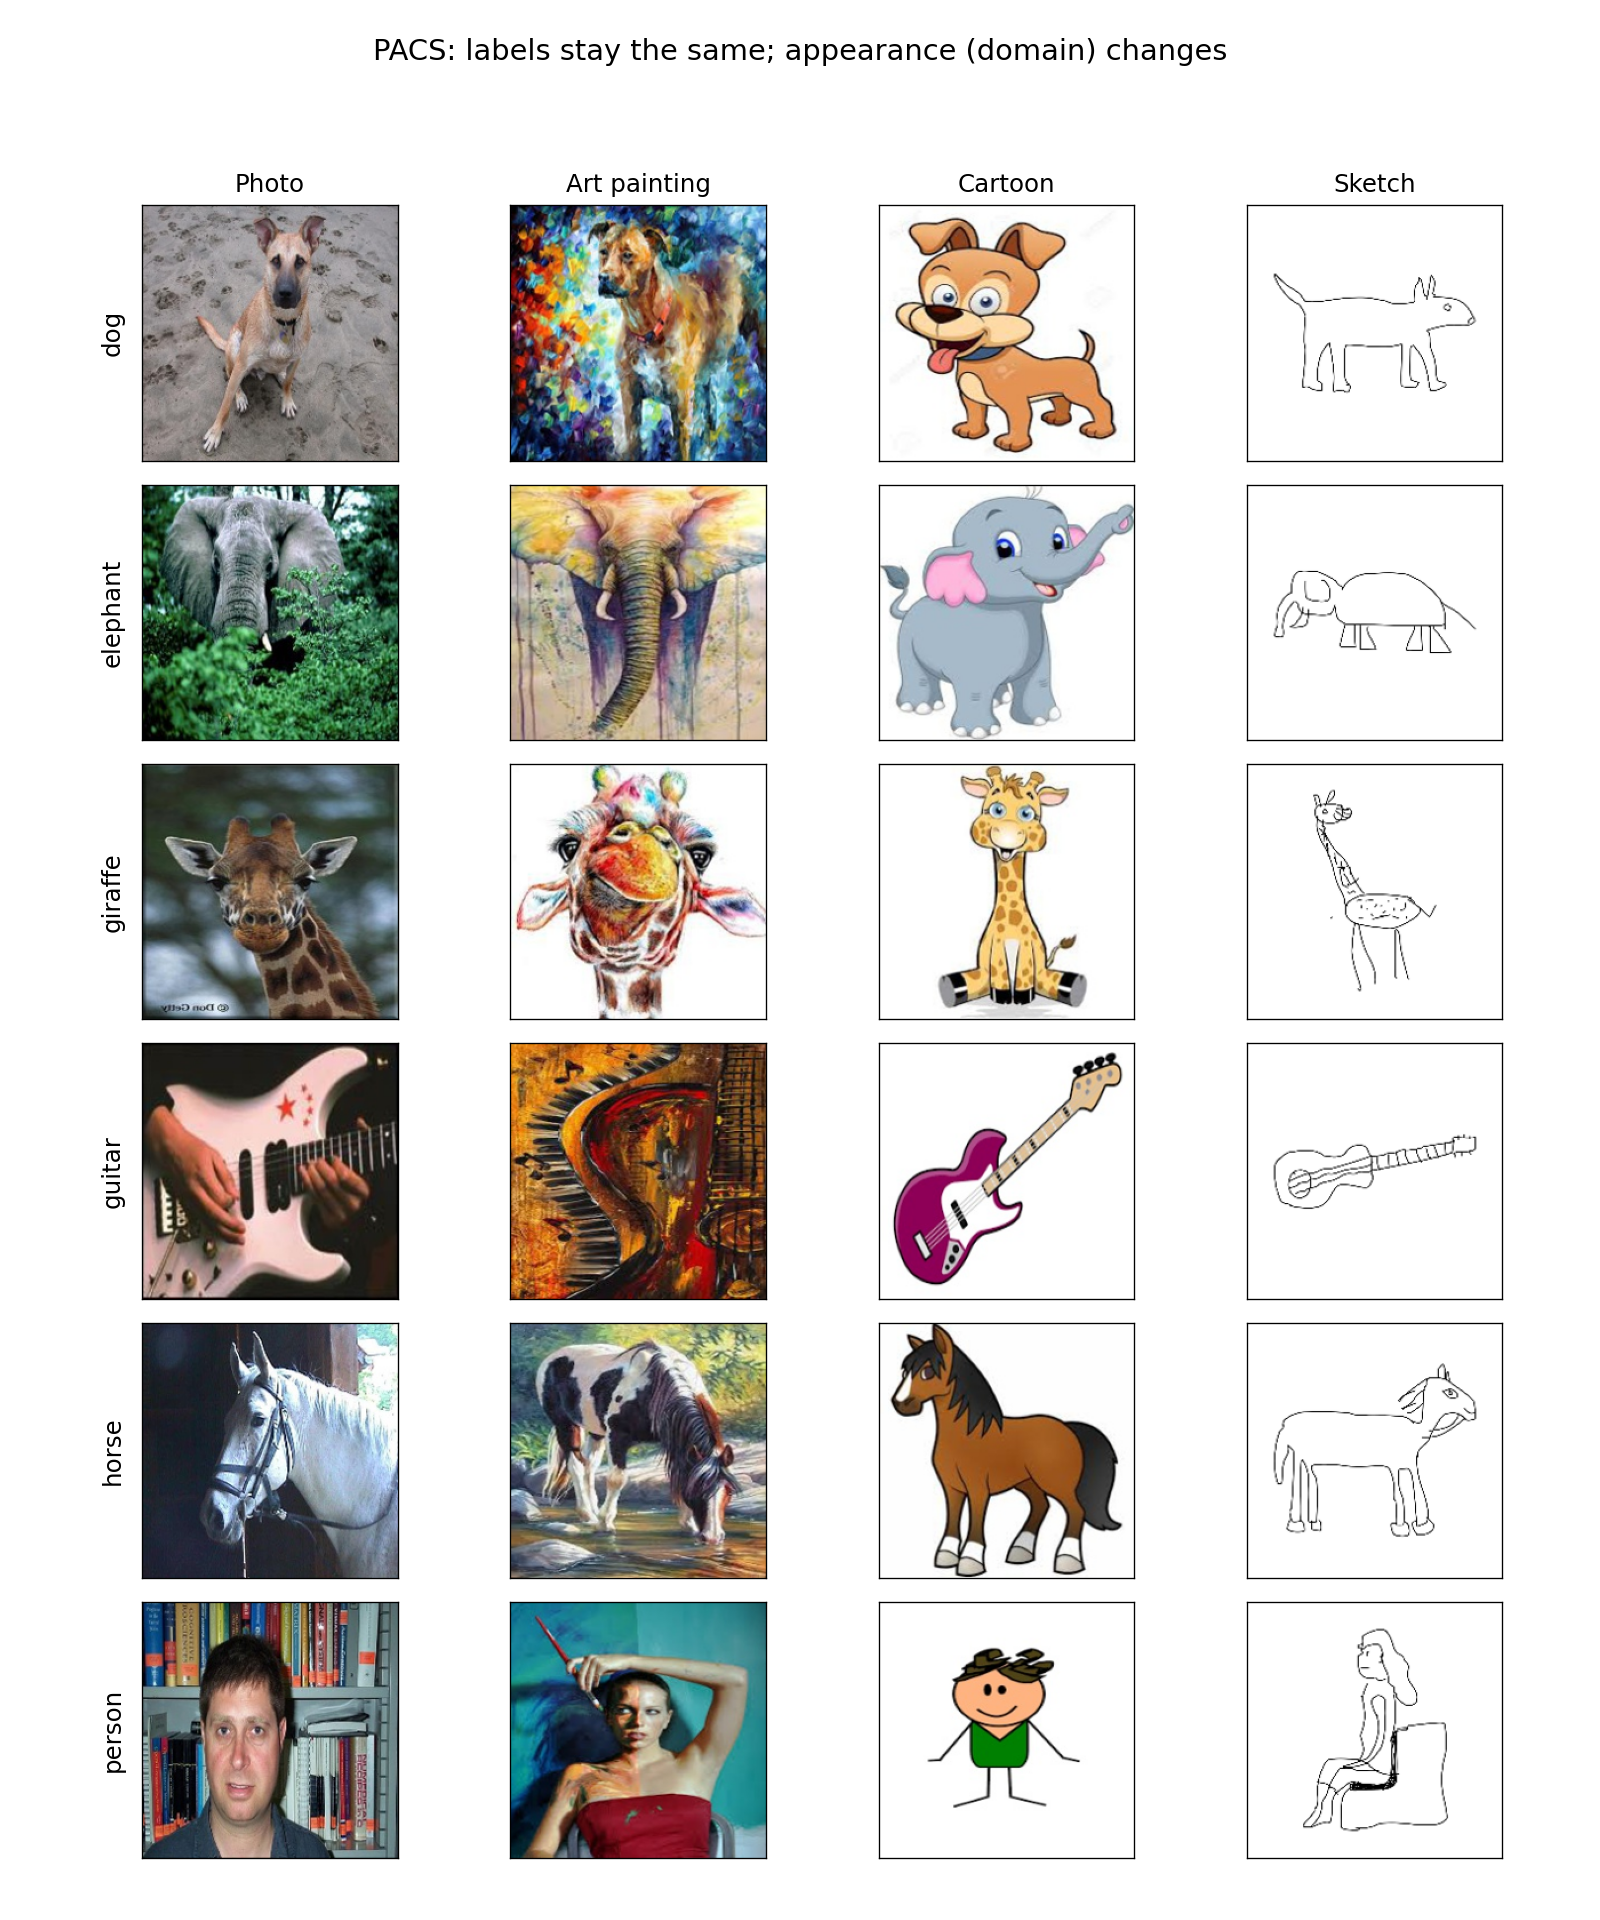
\includegraphics[width=\linewidth]{t2_pacs_classes_across_domains.png}
  \captionof{figure}{PACS classes across Photo, Art, Cartoon, and Sketch.}
  \label{fig:t2_pacs}
\end{minipage}\hfill
\begin{minipage}[t]{0.52\linewidth}
  \captionof{table}{Clean STL-10 subset ($500$ images).
  CLIP-head confidence is low because features are L2-normalized.}
  \label{tab:t1_clean}
  \centering
  \small\setlength{\tabcolsep}{2.5pt}
  \resizebox{\linewidth}{!}{% Auto-generated by report/scripts/make_report_assets.py. Do not edit by hand.
% Sources: task1/results/tables/task1_summary.json
\begin{tabular}{lccc}
\toprule
Model & Top-1 (\%) & Macro-F1 (\%) & Mean max conf. \\
\midrule
ResNet-50 (head) & 97.8 & 97.8 & 0.965 \\
ViT-B/16 (head) & 97.6 & 97.6 & 0.964 \\
CLIP ViT-B/32 (head) & 98.2 & 98.2 & 0.335 \\
CLIP ViT-B/32 (zero-shot) & 96.8 & 96.8 & 0.943 \\
\bottomrule
\end{tabular}
}
  \vspace{8pt}
  \captionof{table}{Translation accuracy / consistency, four-direction mean.}
  \label{tab:t1_translation}
  \centering
  \small\setlength{\tabcolsep}{2.5pt}
  \resizebox{\linewidth}{!}{% Auto-generated by report/scripts/make_report_assets.py. Do not edit by hand.
% Sources: task1/results/tables/task1_summary.json
\begin{tabular}{lcccc}
\toprule
Model & $\delta=0$ & $\delta=8$ & $\delta=16$ & $\delta=32$ \\
\midrule
ResNet-50 (head) & 97.8 / 100.0 & 97.6 / 99.6 & 97.3 / 99.3 & 96.6 / 98.4 \\
ViT-B/16 (head) & 97.6 / 100.0 & 97.6 / 98.4 & 97.4 / 99.0 & 96.5 / 97.5 \\
CLIP ViT-B/32 (head) & 98.2 / 100.0 & 98.0 / 98.6 & 97.7 / 98.0 & 97.5 / 98.0 \\
CLIP ViT-B/32 (zero-shot) & 96.8 / 100.0 & 96.9 / 98.1 & 97.2 / 97.9 & 95.6 / 97.3 \\
\bottomrule
\end{tabular}
}
\end{minipage}

\begin{figure}[H]
  \centering
  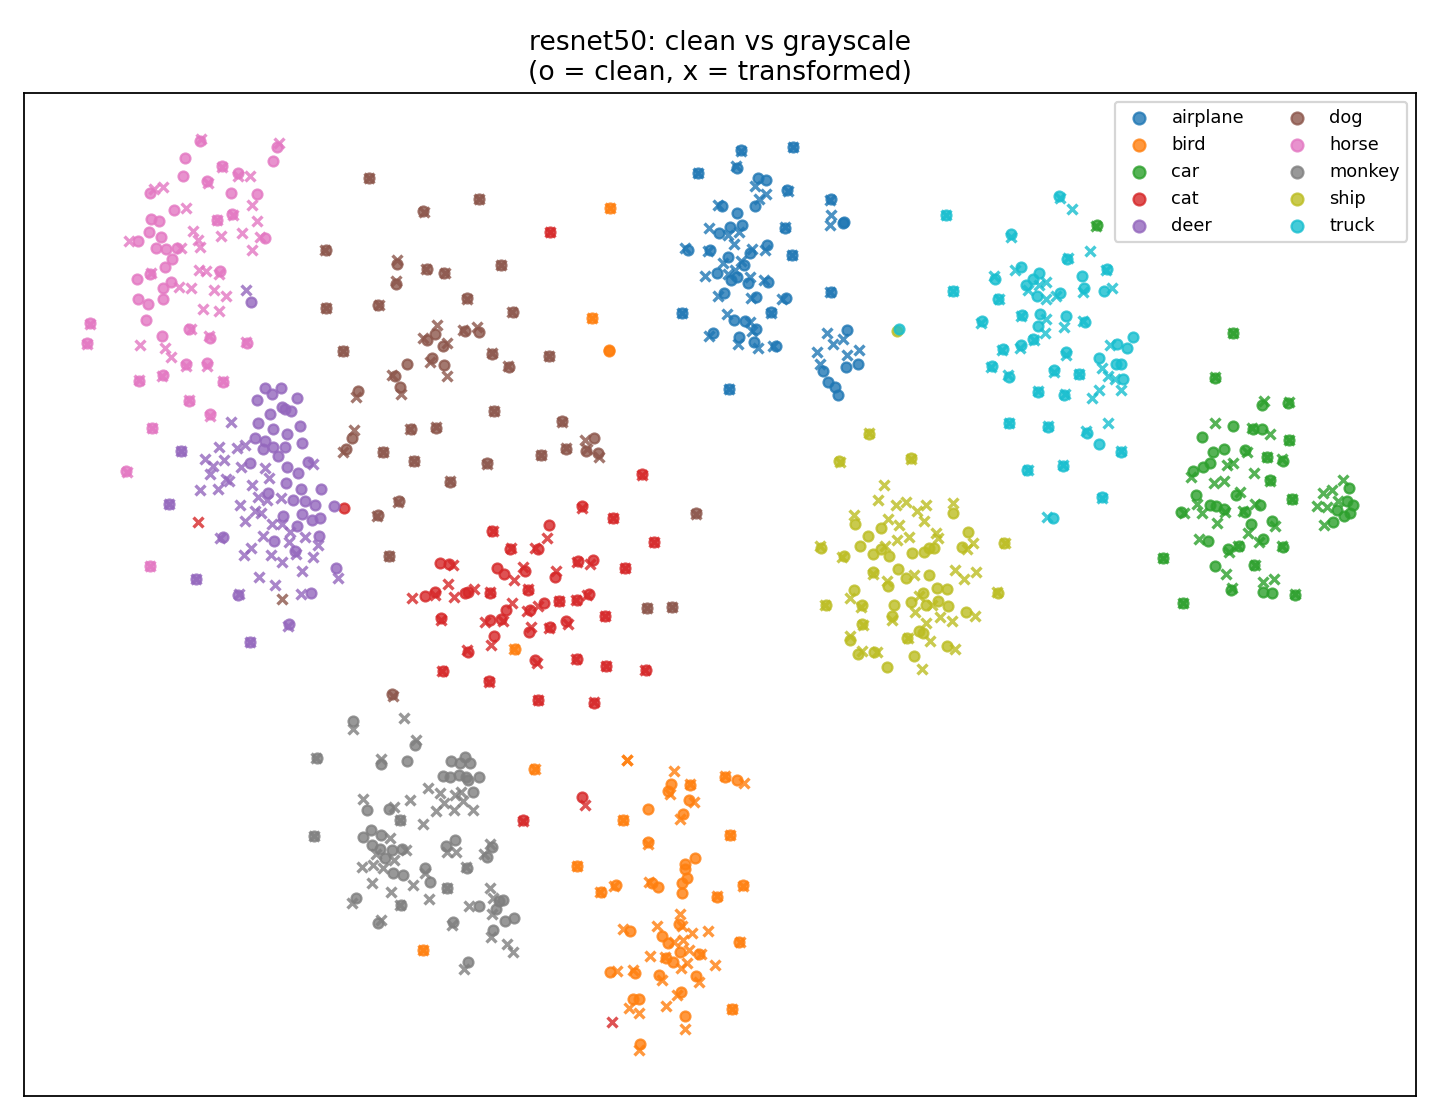
\includegraphics[width=0.32\linewidth]{t1_tsne_resnet50_grayscale.png}\hfill
  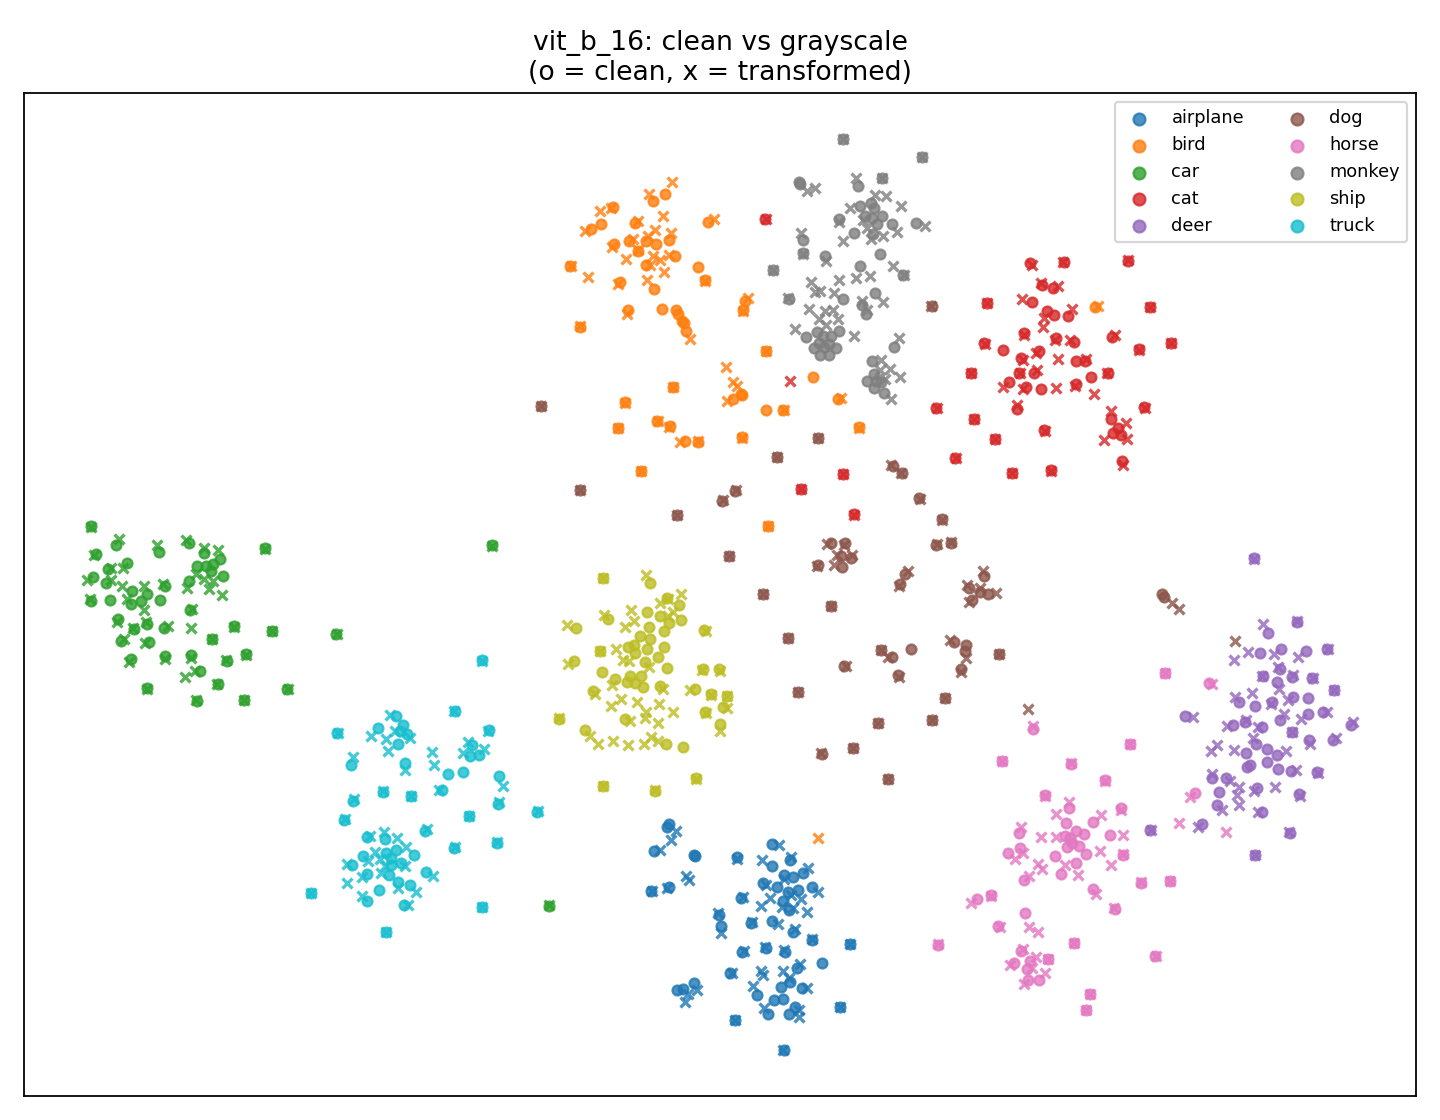
\includegraphics[width=0.32\linewidth]{t1_tsne_vit_grayscale.png}\hfill
  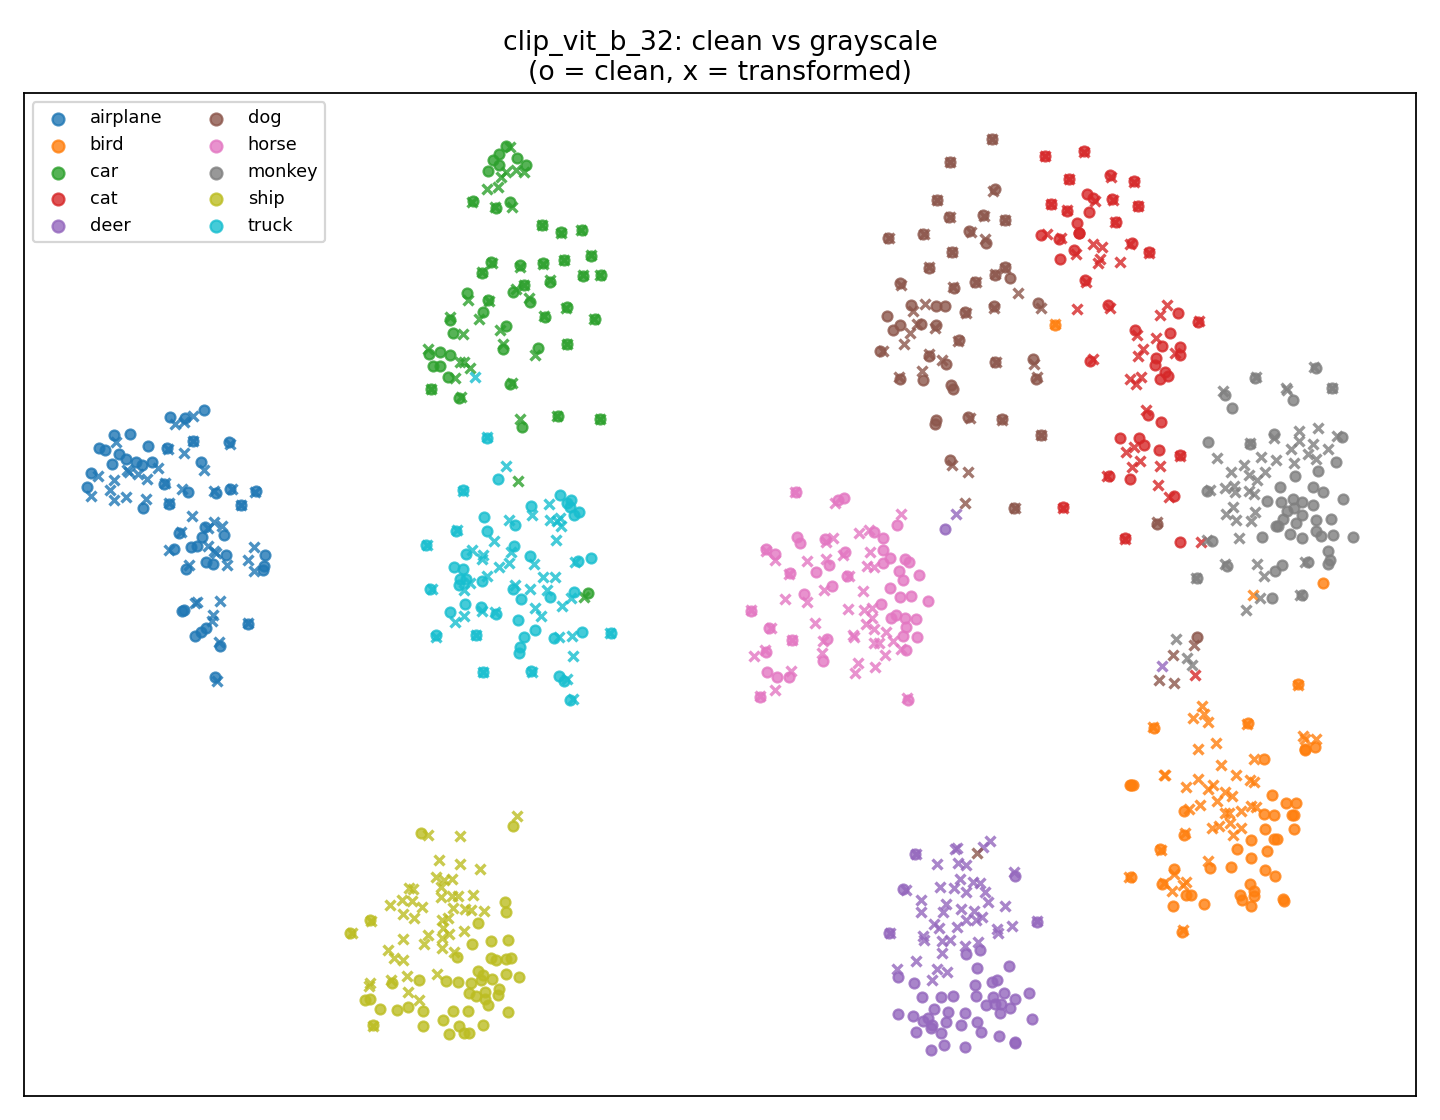
\includegraphics[width=0.32\linewidth]{t1_tsne_clip_grayscale.png}
  \caption{Clean versus grayscale features.
  Class geometry mostly stays; the clouds still shift.}
  \label{fig:t1_tsne_gray}
\end{figure}

\begin{figure}[H]
  \centering
  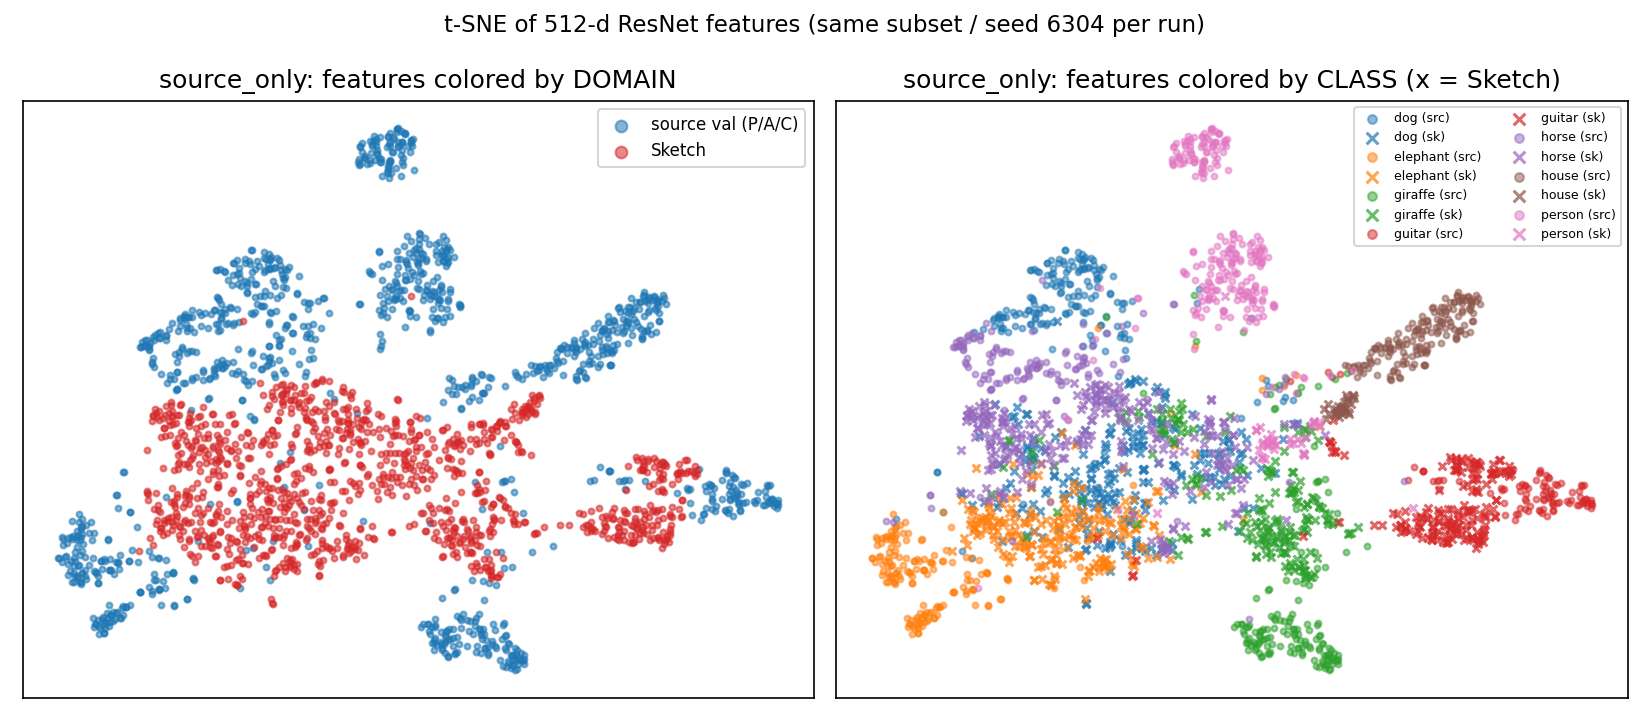
\includegraphics[width=0.49\linewidth]{t2_tsne_source_only.png}\hfill
  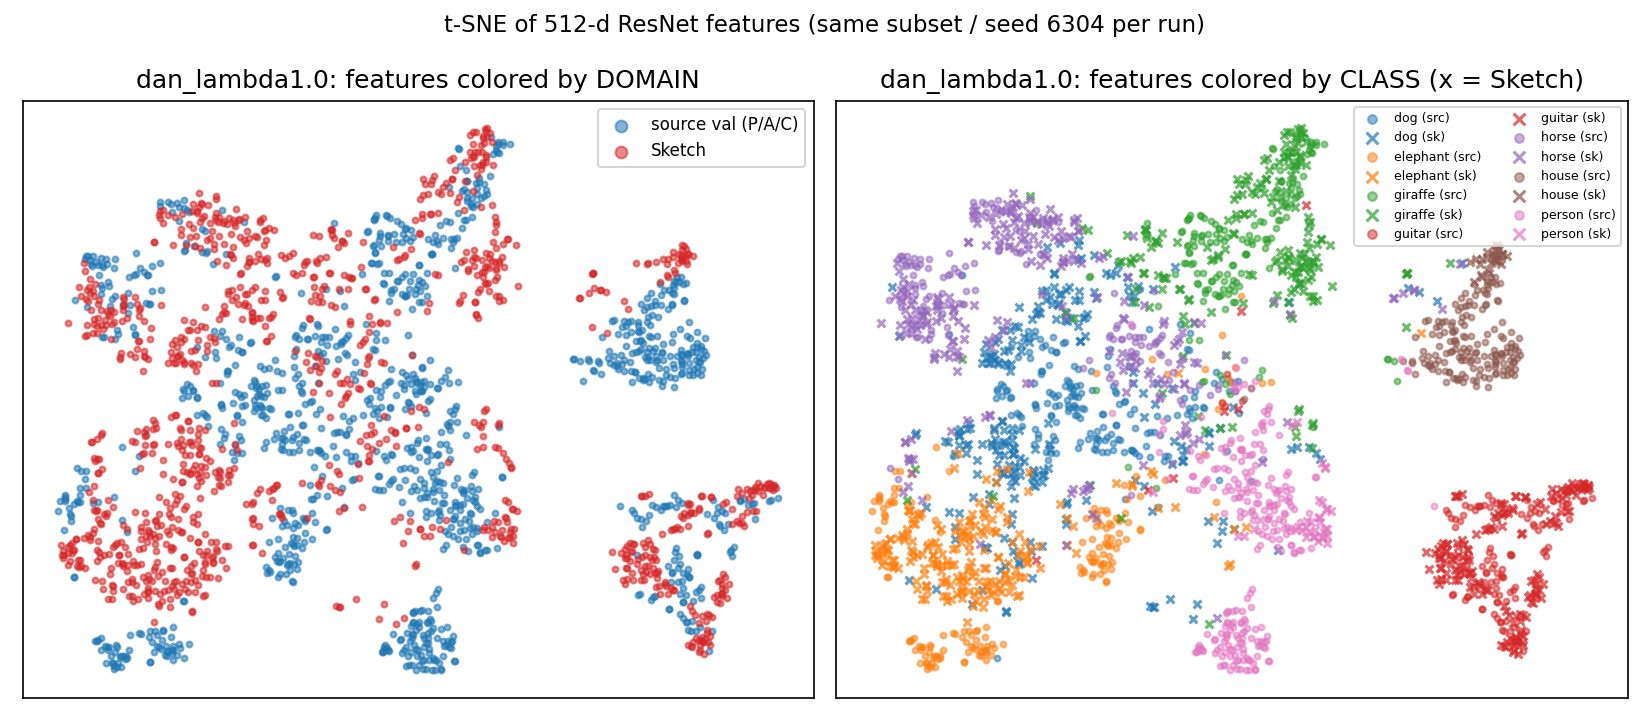
\includegraphics[width=0.49\linewidth]{t2_tsne_dan_lam1.png}\\[2pt]
  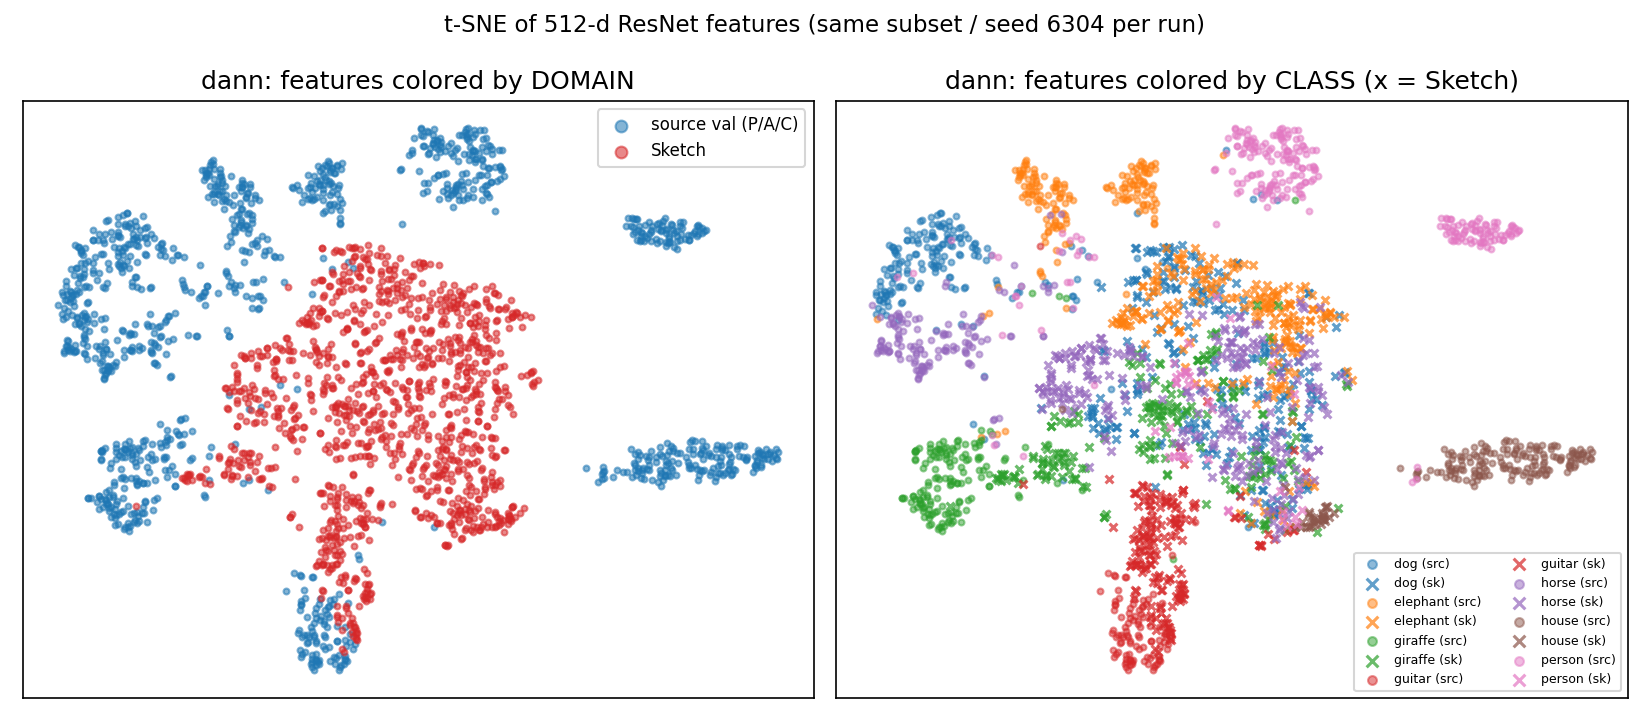
\includegraphics[width=0.49\linewidth]{t2_tsne_dann.png}\hfill
  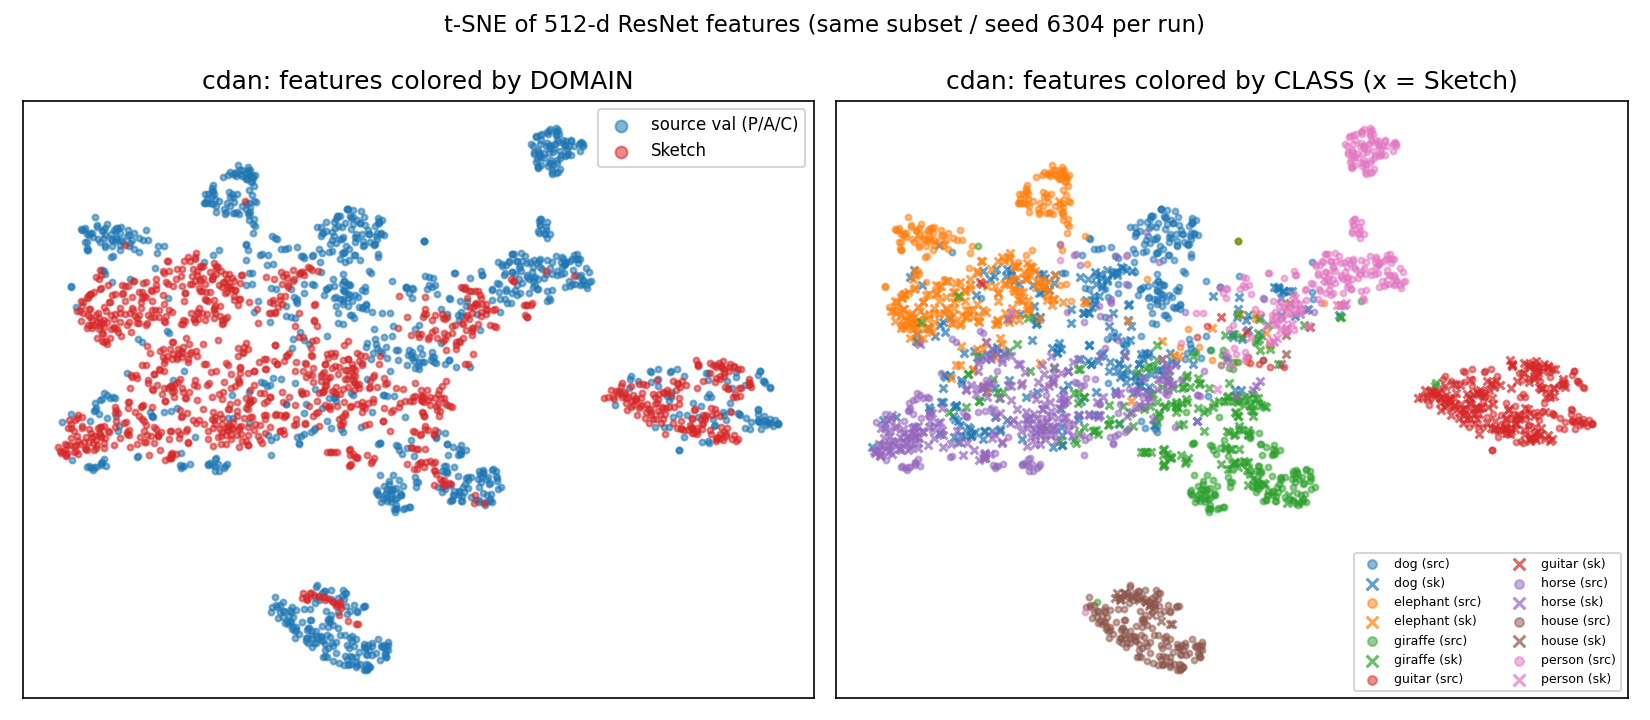
\includegraphics[width=0.49\linewidth]{t2_tsne_cdan.png}
  \caption{Class-colored $512$-d features.
  Top: source-only and DAN $\lambda_{\mathrm{MMD}}=1$.
  Bottom: DANN and CDAN.
  Crosses are Sketch.
  DAN mixes domains and keeps class clouds; DANN isolates Sketch.}
  \label{fig:t2_tsne_so}
  \label{fig:t2_tsne_dann}
\end{figure}

\begin{figure}[H]
  \centering
  \begin{subfigure}[t]{0.38\linewidth}
    \centering
    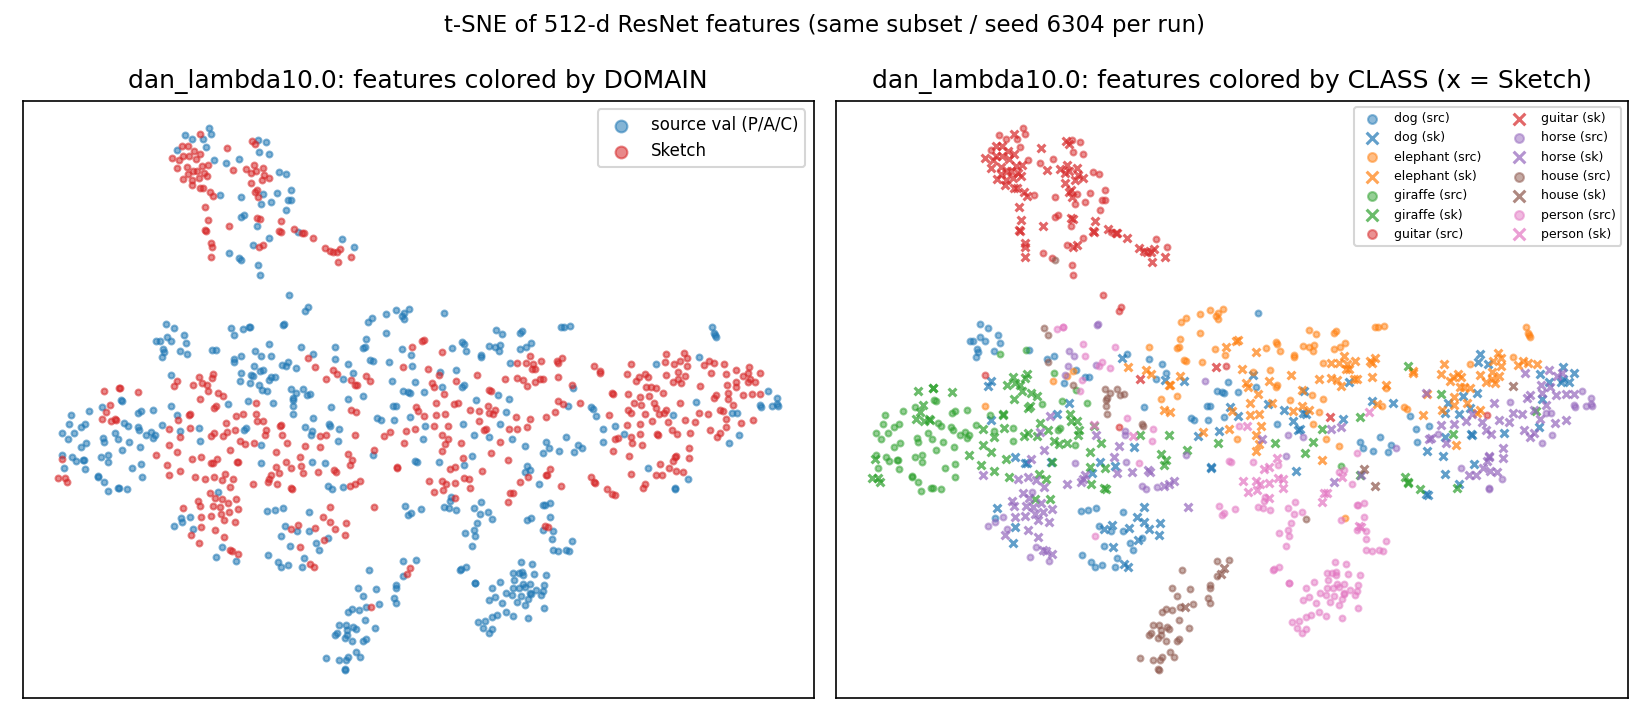
\includegraphics[width=\linewidth]{t2_tsne_dan_lam10.png}
    \caption{DAN $\lambda_{\mathrm{MMD}}=10$.}
    \label{fig:t2_tsne_lam10}
  \end{subfigure}\hfill
  \begin{subfigure}[t]{0.29\linewidth}
    \centering
    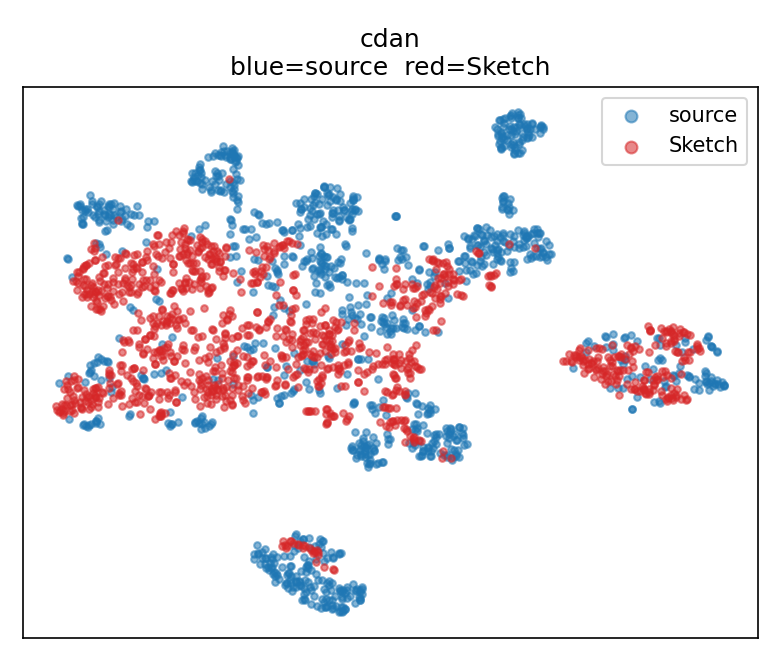
\includegraphics[width=\linewidth]{t2_tsne_domain_cdan.png}
    \caption{CDAN, by domain.}
  \end{subfigure}\hfill
  \begin{subfigure}[t]{0.29\linewidth}
    \centering
    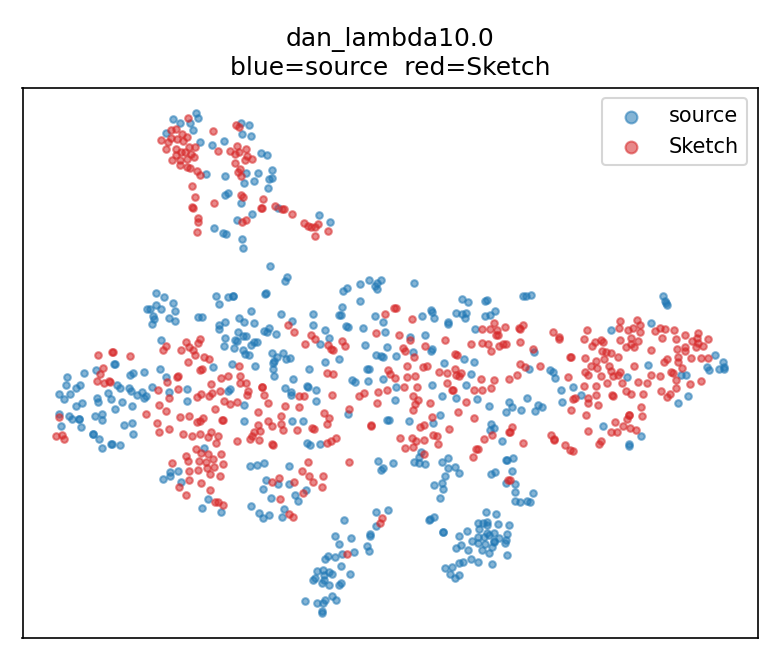
\includegraphics[width=\linewidth]{t2_tsne_domain_dan_lam10.png}
    \caption{DAN $\lambda{=}10$, by domain.}
  \end{subfigure}\\[2pt]
  \begin{subfigure}[t]{0.49\linewidth}
    \centering
    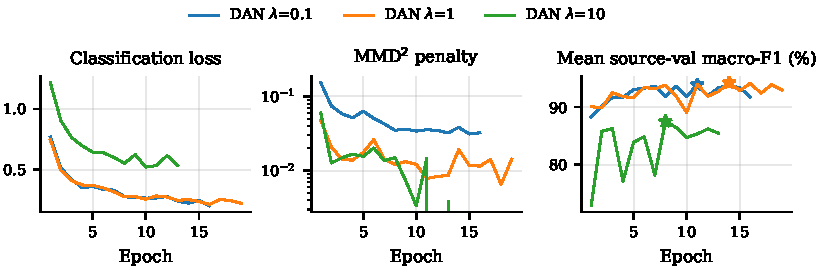
\includegraphics[width=\linewidth]{t2_lambda_curves.pdf}
    \caption{DAN $\lambda$ training.}
    \label{fig:t2_lambda_curves}
  \end{subfigure}\hfill
  \begin{subfigure}[t]{0.49\linewidth}
    \centering
    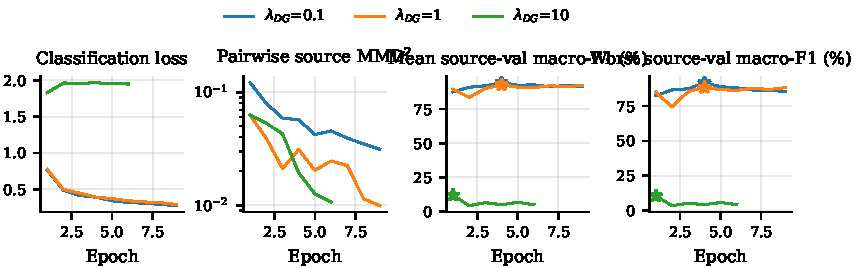
\includegraphics[width=\linewidth]{t3_lambda_curves.pdf}
    \caption{DAN-DG $\lambda_{\mathrm{DG}}$ training.}
    \label{fig:t3_lambda_curves}
  \end{subfigure}\\[2pt]
  \begin{subfigure}[t]{0.49\linewidth}
    \centering
    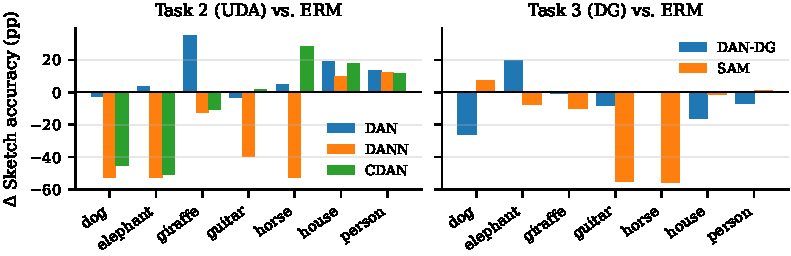
\includegraphics[width=\linewidth]{t23_perclass_delta.pdf}
    \caption{Per-class Sketch change versus ERM.}
    \label{fig:perclass_delta}
  \end{subfigure}\hfill
  \begin{subfigure}[t]{0.49\linewidth}
    \centering
    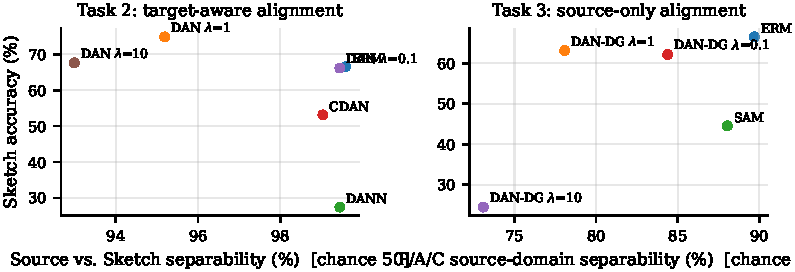
\includegraphics[width=\linewidth]{t23_separability_vs_sketch.pdf}
    \caption{Domain probe versus Sketch accuracy.}
    \label{fig:sep_vs_sketch}
  \end{subfigure}
  \caption{Leftover $\lambda$ embeddings, training curves, per-class Sketch change, and the domain-probe plot.}
\end{figure}

\end{document}
